Behavioral watchpoint provides an efficient software-based watchpoint framework that simplifies the implementation of DBT-based program analysis and debugging tools. This chapter describes the design of behavioral watchpoints and the various features enabled by our design. We present the challenges raised by our approach and then describe our implementation of behavioral watchpoints. 
%Behavioral watchpoint leverages the advances in binary instrumentation and code manipulation tool to provide an efficient debugging framework that can substantially increase the feature set of standard off the shelf debuggers. 
Two characteristics that defines the watchpoints are:
\begin{enumerate}[i)]
	\item Context-specific information is embedded in each watchpoint. This information is directly available when a watched address is accessed, providing significant versatility in monitoring a large number of memory addresses.
	%\item The action taken when a watched address is accessed is a component of the context-specific information. This implies that different watchpoints can \emph{behave} differently.
	\item A behavioral watchpoint watches a \emph{range} of addresses, enabling object-granularity watchpoints, i.e., one watchpoint can watch an entire object or memory block.
%watchpoints. This enables the feature where one watchpoint can watch the entire object or memory block.%(i.e., one watchpoint watches an entire object). 
\end{enumerate}



%. This design supports our goal of allowing one watchpoint to monitor all memory accesses to a single object.

%To achieve this design goal, we implemented
\section{Design}\label{sec:design}
The design of the behavioral watchpoint framework is motivated by our aim to provide context-specific information on memory accesses, which helps provide significant versatility when monitoring these accesses. This context specific information is stored in an in-memory data structure and accessed before memory read/write operations. %which is referred before every read/write operations on memory blocks. and accessed before memory read/write operations. 
%
%
Our design is based on the key observation that the pointers in 64 bit architectures have spare bits. Both AMD64 and Intel x86-64 processors use a 48 bit implementation leaving 16 spare bits that can be used to store pointer metadata information. 
%which can be used to store the information about the pointers.

We implement watchpoints by adding an extra level of indirection to memory addresses. An unwatched address is converted into a watched address by changing its spare high-order bits. The high order bits of an unwatched address have the value \texttt{0xffff}. We call this value the canonical value. For watched addresses, the high-order bits are converted to a non-canonical value that helps identify context-specific information about the range of memory being watched. This information, called the watchpoint's \emph{descriptor}, contains the originating watched address, meta-information and a set of functions (\emph{vtable}) to invoke when watched memory is dereferenced. Since watchpoint information is embedded in the high-order bits, a typical offset of a watched address is another watched address that shares the same descriptor. 

The design of behavioral watchpoints is shown in \Figref{watchpoint_descriptor_table}. Our design uses 15 high-order bits (called the \emph{counter index}) and an additional 8 bits (bits 20-27, called the \emph{inherited index}) of a watched address to identify the index into a global \emph{watchpoint descriptor table}. The \emph{watchpoint descriptor table} stores a pointer to the watchpoint's descriptor. The key advantage of our design scheme is i) the ability to map watched addresses to unwatched addresses using a simple bitmask and  ii) the ability to easily access a watchpoint's descriptor when a watched address is accessed. The high-order 15 bits counter index allows us to use 32K watchpoints at a time and the additional 8 bits of inherited index extends the number of possible watchpoints to 8M. The inherited index is left unchanged when converting an unwatched address into watched.

However, one drawback of our design is that an offset of a watched address can cause the low-order bits to overflow into the inherited index and this will lead a watched address to point to an incorrect descriptor. One approach to deal with this issue is to assign  multiple descriptors for the watched objects holding the same meta-information and putting them in adjacent indices or duplicating the same descriptor entry across adjacent indices. This is possible because inherited indexes make the descriptor table more sparse allowing them to have duplicate entries.


%15 bits only allows 32K watchpoints. To increase the number of watchpoints, we use
%an additional 8 bits (bits 20-27, called the counter index)
%in the address to index into the watchpoint descriptor table (Figure 1). This counter index  and is left unchanged when
%converting an unwatched address into a watched address.
%The key advantage of our watchpoint scheme is the ability to directly map watched addresses to unwatched addresses using a simple bitmask. The main drawback of
%the scheme is that an offset of a watched address can  


%e 48 out of 64 bits in pointers,
%and Windows further limit this to 43 bits for user space
%programs. Thus 21 bits in the pointer representation are
%not used. Next we describe two uses for these spare bits,
%and present a performance evaluation on AMD64.

%Behavioral watchpoints is designed by adding an extra level of indirection to memory addresses. An unwatched address is converted into a watched address by changing its high-order bits. These high-order bits indirectly identify context-specific information about the range of memory being watched. This information, called the watchpoint's \emph{descriptor}, contains the originating watched address, meta-information and a set of functions (\emph{vtable}) to invoke when watched memory is dereferenced. Since watchpoint information is embedded in the high-order bits, a typical offset of a watched address is another watched address that shares the same descriptor. 

\begin{figure}[t]
\begin{center}
%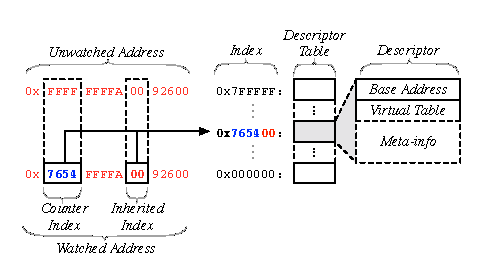
\epsfig{file=watchpoints.eps, width=3.0in, height=1.4in}
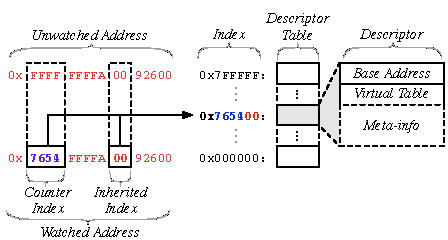
\includegraphics[width=6.0in]{watchpoints.pdf}
\end{center}
\vspace{-15pt}
\caption[Design of behavioral watchpoints.]{\label{fig:watchpoint_descriptor_table}A watched address (bottom left) and its corresponding unwatched address (top left) are compared. The watched address takes the form of non-canonical address that are not addressable in kernel space. The watchpoint framework uses a \emph{counter index} and an \emph{inherited index} to store the descriptor information in a global descriptor table. The process of resolving the watchpoint descriptor is shown.}
%for the watched address is shown.}
\end{figure}


Our design of behavioral watchpoints is geared to the 64 bit x86 (x86-64) architecture. In kernel space on the x86-64 architecture, the addressable memory includes the canonical form of addresses with their 16 high-order bits set to 1. Tagging these higher order bits with the descriptor information converts them to a non-canonical address that triggers a hardware exception when dereferenced. The watchpoint framework takes advantage of the exception to implement behavioral watchpoints.

%The design of behavioral watchpoint is shown in \Figref{watchpoint_descriptor_table}. It uses 15 high-order bits (called the \emph{counter index}) and an additional 8 bits (bits 20-27, called the \emph{inherited index}) of a watched address to identify the index into a global \emph{watchpoint descriptor table} which stores the pointer to the watchpoint's descriptor. %This extends the number of possible watchpoints to 8M. 
%The key advantage of our watchpoint scheme is the ability to directly map watched addresses to unwatched addresses using a simple bitmask. One drawback of the scheme is that an offset of a watched address can cause the low-order bits to overflow into the inherited index. We overcome this issue by assigning multiple descriptors for the watched objects holding the same meta-information and by putting them in adjacent indices. 

%is to manage multiple descriptors for a watched object.

%The watched addresses are non-canonical addresses that trigger a hardware exception when dereferenced. 
%We take advantage of the x86-64 architecture for implementing watched addresses. In kernel space on x86-64, canonical addresses have their 16 high-order bits set to 1. Watched addresses do not take this form; they are non-cannonical addresses that trigger a hardware exception when dereferenced. 
Our watchpoint framework uses two approaches to perform memory operations on watched objects. First, when watchpoints are expected to be triggered frequently, it dynamically adds instrumentation at every memory load and store to avoid hardware exceptions. Watched addresses are detected before they are dereferenced and resolved to their unwatched counterparts (by masking the 16 high-order bits to 1). The approach is called code-centric instrumentation because the decision about the code translation and instrumentation is taken based on the execution path. 
Second, when watchpoints are unlikely to be triggered, the alternative approach is to dereference a watched address and implement behavioral watchpoints in the trap handler. This enables on-demand binary translation and allows adding instrumentation only when a watchpoint is triggered. We call this approach data-centric instrumentation because code translation and instrumentation is based on watchpoint accesses.


%We call it the data-centric instrumentation which enables the feature of adding selective instrumentation. The approach takes decision about code translation and instrumentation based on the access of watchpoints. 


%, which lowers the overhead of binary translation. % when watchpoints are fewer in number and unlikely to be triggered. 

The design of behavioral watchpoints provides the following benefits:
\begin{enumerate}[i)]
\item \emph{\textbf{Multiple watchpoints can watch the same range of memory:}} 
Two copies of an address (e.g., two pointers to the same object) can be watched separately, so long as the high-order bits index different entries in the watchpoint descriptor table. %they manage different descriptors. 
This is useful for distinguishing between logically different objects that occupy the same memory region. For example, this enables efficient detection of use-after-free bugs without preventing deallocated memory from being immediately reallocated for another use. This efficiency comes from our ability to have one watchpoint for the freed object and another watchpoint for the newly allocated memory occupying the same space.

\item \emph{\textbf{Watchpoint descriptors are context specific:}} 
Our design separates the allocation and management of descriptors from the watchpoint framework. It is the responsibility of each client to manage its descriptors. When a watchpoint gets added to an object, the client determines the \emph{vtable}, \emph{type} and \emph{meta-information} that needs to be stored in the descriptor, as shown in \Figref{watchpoint_descriptor_table}. The vtable determines the function that is invoked when watched memory is accessed. Each vtable provides eight functions: four read and four write functions. Each function is specific to a memory operand size (1, 2, 4, or 8 bytes). A watchpoint descriptor is initialised with either a generic or a type-specific vtable, which is specific to the \emph{type} of the watched address. The meta-information allows the descriptors to be arbitrarily customized or extended based on the needs of the client.

\item \emph{\textbf{Watchpoints are viral:}}
Behavioral watchpoints can be used virally. If an address $A$ is watched, then every address derived from $A$ (e.g., through copying or offsetting) is also watched. This is useful for memory and taint analysis tools. For instance, a watchpoint that is added early in the lifetime of an address (e.g., immediately before the address of newly allocated memory is returned from an allocator) can persist and propagate until no more derived addresses exist.
\end{enumerate}

%Behavioral watchpoints earn their name from vtable because they allow watchpoints to behave differently when watched memory is accessed.


%A watchpoint's descriptor is indirectly located by interpreting these high-order bits as an index into a global \emph{watchpoint descriptor table} which stores the pointer to watchpoint's descriptor(\Figref{watchpoint_descriptor_table}). 
%Because these bits do not change, many addresses end up indirectly referring to the same watchpoint descriptor.

%\subsection{Design Implications}
%Our approach has the following design implications.

%Any unwatched address can be converted into an watched address. The extra level of indirection added by watching an address allows us to efficiently locate context-specific information about the memory being watched.

%A watchpoint is added to a program by changing the high-order order bits of an address used by the program. 
%Watchpoints work on ranges instead of individual units of memory because a watchpoint is added to a program by changing 

%\paragraph{A watched address must be distinguishable from an unwatched address.} 

%Behavioral watchpoint framework provides API \emph{add\_watchpoints()} which is used to add watchpoints to an arbitrory object. It takes the obeject address and size to creates the descriptor for the object. The descriptor can be based on the type or size of the object. The descriptor can be changed dynamically if required. The descriptor is then stored into descriptor table at the next free index generated by counter and partial index. If some object doesn't need descriptor they are only assigned the watched address with corrosponding index in the descriptor table assigned NULL. 

%Behavioral watchpoint provides support where two copies of an address (e.g., two pointers to the same object) can be separately watched, so long as they manage different descriptors, the high-order bits index different entries in the watchpoint descriptor table. 
%This is useful for distinguishing between logically different objects that occupy the same memory. For example, this feature enables efficient detection of use-after-free bugs without preventing deallocated memory from being immediately reallocated for another use. This efficiency comes from our ability to have one watchpoint for the freed memory, and another watchpoint for newly allocated memory occupying the same space.


%\paragraph{Multiple watchpoints can watch the same range of memory.} Two copies of an address (e.g., two pointers to the same object) can be separately watched, so long as they manage different descriptors. %the high-order bits index different entries in the watchpoint descriptor table. 
%This is useful for distinguishing between logicallywatchpoint framework  different objects that occupy the same memory. For example, this feature enables efficient detection of use-after-free bugs without preventing deallocated memory from being immediately reallocated for another use. This efficiency comes from our ability to have one watchpoint for the freed memory, and another watchpoint for newly allocated memory occupying the same space.

%\paragraph{Millions of watchpoints are supported.} Our design as described uses 15 high-order bits (called the \emph{counter index}) and additional 8 bits (bits 20-27, called the \emph{inherited index}) of a watched address for identifying a watchpoint's descriptor.  This extends the number of possible watchpoints to 8M.  %and is left unchanged when converting an unwatched address into a watched address.
%The key advantage of our watchpoint scheme is the ability to directly map watched addresses to unwatched addresses using a simple bitmask. The main drawback of the scheme is that an offset of a watched address can cause the low-order bits to overflow into the inherited index. One solution to overcome this problem is to manage multiple descriptors for a watched object. 

%Our design allows the same range of memory to be watched differently. For example, two pointers to the same object can be watched separately, so long as they manage different descriptors. This feature is useful for distinguishing logically different objects that occupy the same memory. For example, this feature enables efficient detection of use-after-free bugs without preventing deallocated memory from being immediately reallocated for use. Having one watchpoint for the freed memory, and another watchpoint for newly allocated memory occupying the same space, is critical for this application. %Watchpoint gets added with a call to \texttt{ADD\_WATCHPOINT} which takes the reference of object and corrosponding meta-information as parameter. \texttt{REMOVE\_WATCHPOINT} is used to remove watchpoint from a watched object. 

%For example, this feature enables efficient detection of use-after-free bugs without preventing deallocated memory from being immediately reallocated for another use. This efficiency comes from our ability to have one watchpoint for the freed memory, and another watchpoint for newly allocated memory occupying the same space.

%We are exploring several solutions to this problem.

% This counter index extends the number of possible watchpoints to 8M and is left unchanged when converting an unwatched address into a watched address. The key advantage of our watchpoint scheme is the ability to directly map watched addresses to unwatched addresses using a simple bitmask. The main drawback of the scheme is that an offset of a watched address can cause the low-order bits to overflow into the counter index. We are exploring several solutions to this problem.

% and 8 bits (bits 20-27, called the \emph{inherited index}) for identifying a watchpoint's descriptor

%of a watched address for identifying a watchpoint's descriptor. 15 bits only allows 32K watchpoints. To increase the number of watchpoints, we use an additional 8 bits (bits 20-27, called the \emph{inherited index}) in the address to index into the watchpoint descriptor table (\Figref{watchpoint_descriptor_table}). This counter index extends the number of possible watchpoints to 8M and is left unchanged when converting an unwatched address into a watched address. The key advantage of our watchpoint scheme is the ability to directly map watched addresses to unwatched addresses using a simple bitmask. The main drawback of the scheme is that an offset of a watched address can cause the low-order bits to overflow into the counter index. We are exploring several solutions to this problem.

%\paragraph{Millions of watchpoints are supported.} Our design as described uses 15 of the 16 high-order bits (called the \emph{counter index}) of a watched address for identifying a watchpoint's descriptor. 15 bits only allows 32K watchpoints. To increase the number of watchpoints, we use an additional 8 bits (bits 20-27, called the \emph{inherited index}) in the address to index into the watchpoint descriptor table (\Figref{watchpoint_descriptor_table}). This counter index extends the number of possible watchpoints to 8M and is left unchanged when converting an unwatched address into a watched address. The key advantage of our watchpoint scheme is the ability to directly map watched addresses to unwatched addresses using a simple bitmask. The main drawback of the scheme is that an offset of a watched address can cause the low-order bits to overflow into the counter index. We are exploring several solutions to this problem.

%This approach has some drawbacks when an offset of a watched address causes the low-order bits to overflow into the counter index; however, we have several solutions to this problem. 

%\paragraph{Watchpoint descriptors are context-specific.} Our design separates the allocation and management of descriptors from the watchpoint framework. It is the responsibility of each client to manage its descriptors. %, which % and declare the corrosponding descriptor type for the framework. provides complete flexibility in handling it. 
%When a watchpoint gets added to an object, the client determines the \emph{type}, \emph{meta-information} and \emph{vtable} which needs to be stored in the descriptor. These descriptors can be arbitrarily customized or extended based on the needs of the client. %One powerful application of this extension is discussed in section~\ref{sec:access_policies}.




%This aspect of watchpoints is possible because our design separates the allocation/management of descriptors and the addresses that they watch. When a watchpoint is added to an address, the \emph{type} or \emph{size} of the address determines what meta-information is included in the descriptor, as well as what function to invoke when memory watched by the watchpoint is accessed. These descriptors can be arbitrary customized or extended based on the needs of program analysis tools. Two powerful applications of this extension are discussed in \Secref{type_overflow} and \Secref{access_policies}.


%Arbitrary extension of descriptors supports our goal of overcoming the incongruency between the needs of debugging an analysis tools (contextual information about watched memory), and how existing software implements watchpoints (watched memory is opaque).

%\subsection{Extensions}
%Our design includes the following extensions to watchpoints, which expand on the behavioral aspect of our watchpoint implementation.
%principally enable the \emph{behavioral} aspect of our software-based watchpoint .
%Our goal of using watchpoints to watch the memory of objects required the following 

%\paragraph{Watchpoints are type-specific.} When a watchpoint is added to an address, the \emph{type} of the address determines what meta-information is included in the descriptor, as well as what functions to invoke when memory watched by the watchpoint is accessed. Two powerful applications of this extension are discussed in \Secref{type_overflow} and \Secref{access_policies}.

%\paragraph{Triggered watchpoint functions are polymorphic.} The function invoked when watched memory is accessed is decided using a descriptor-specific \emph{vtable}. Each vtable provides eight functions: four read and four write functions. Each function is specific to a memory operand size (1, 2, 4, or 8 bytes). A watchpoint descriptor is initialised with either a generic or a type-specific vtable, which is specific to the \emph{type} of the watched address. %Behavioral watchpoints earn their name from vtable because they allow watchpoints to behave differently when watched memory is accessed.

%When invoked, a vtable function operates on the watched address and its descriptor. Behavioral watchpoints earn their name from their ability to behave differently based on the meta-information stored in the descriptor and the (type-specific) vtable function invoked.

%\paragraph{Watchpoints remember their originating address.} The address to which a watchpoint is first added is called its \emph{base address}, and is stored in the watchpoint descriptor. We designed watchpoints to remember their base address because it helps to ``anchor" contextual information. When a watchpoint is added, \emph{something} is known about the watched address. Later in a program's execution, an offset of the watched address might be dereferenced. Little can be said about the dereferenced address in relation to the watchpoint's originating address without knowing the originating address.

%Without the former context of why or where the watchpoint was originally added, there is little that can be said about the relation between the triggered address and 
%the watched memory except that it might be arbitrarily far away from the address to which the watchpoint was originally added.
%That is, something is known about an address when the decision to add a watchpoint to that address is made. 
%If the original address is not remembered, then it is difficult to relate a triggered watchpoint
%We designed watchpoints this way so that at any point during the lifetime of a watchpoint, 
%Watchpoints were designed this way so that contextual information is always ``anchored" to something that was once known. 

%This is consistent with our goal of using watchpoints to watch the memory of an object because we expect the base address to be the address in memory of a watched object.

%Watchpoint desc

%Because watchpoints are added to addresses, and 

%This means that 


%We can change an address into a \emph{watched address} by ensuring that a watched address is non-canonical: it cannot legally be used (on x86) without triggering a hardware exception.


%changing part of an address, not by 
%The watched range is \emph{anchored} on the address on which the watchpoint is initially added (called the base address). 

%Behavioral watchpoints are implemented by changing an address to-be-watched into a non-canonical address\footnote{In kernel space on x86, a canonical virtual address has its 16 high-order bits set to 1. Current x86 processors require that the 8 high-order bits of an address match the $9^{th}$ highest order bit.}. The translation from unwatched to watched alters the unused high-order bits of an address. 

%There are several implications of this design decision:
%\begin{enumerate}
%	\item 
%\end{enumerate}



%Behavioral watchpoints were designed with the following goals in mind:
%\begin{enumerate}
%	\item 
%\end{enumerate}

%\subsection{Design Challenges}
%The design of behavioral watchpoint put following restrictions in the way it can be used:
%\begin{enumerate*}
%\item[i)] A watchpoint must be added at the object source. Adding watchpoints at arbitrary location must be avoided since there is a possibility of another unwatched copy of the same object existing in the program data. This will introduce incosistency and object will be partially watched.
%\item[ii)] Behavioral watchpoints can't be used in applications playing with high-order bits. Such operation will introduce incosistency in descriptor information attached with watched addresses. Applications doing similar things like depending on sign-extension of the 64-bit addresses or handling of 32-bit addresses is also not supported. Identifying and ignoring such cases is a problem and we are exploring solutions to this.
%\item[iii)] Behavioral watchpoints are implemented for Linux kernel and one should be careful when using page-table lookup for watched addresses. Operations such as \texttt{\_\_pfn\_to\_page} and \texttt{\_\_page\_to\_pfn} can lead to wrong \texttt{page} structure or loss of descriptor information.
%One should also be careful when using kernel functions for page-table lookup on watched addresses.
%We found some cases where fast method of mapping virtual addresses to physical addresses for page table lookup was depending on sign extension of 64-bit addresses which is not the case when it is changed to watched addresses. 

 %can't be used in applications playing with high-order bits. Such operation will introduce incosistency in descriptor information attached with watched addresses. Applications doing similar things like depending on sign-extension of the 64-bit addresses or handling of 32-bit addresses is also not supported. Identifying and ignoring such cases is a problem and we are exploring solutions to this.
%\end{enumerate*} 

%put some restrictions on the range of applications which it can handle. Behavioral watchpoint tags the higer-order bits with the descriptor information and it can't handle the application which is also doing similar things. Such operation will corrupt the embedded descriptor information and once lost we don't have a way to recover it. Identifying applications doing such operation is challenging. Applications which are only handling with 32-bit address is also not supported. We designed behavioral watchpoints for the Linux kernel but all the functionalities in the kernel is not very suitable for the approach. We found some cases where fast method of mapping virtual addresses to physical addresses for page table lookup was depending on sign extension of 64-bit addresses which is not the case when it is changed to watched addresses. 

%has the following design implications. 

%are designed for Linux kernel and generated by providing an extra-level of indirection and storing the descriptor information in higher order bits of the address. This puts restrictions on the range of applications which behavioral watchpoints can handle. The applications storing tagging information with the high-order bits of the address works against the design of behavioral watchpoints. Identifying such operations in an application is an open problem for us. Our solution of embedding descriptor information in object address is not very friendly with some of the kernel functions.   


%However identifying such operations in an application is an  


%However all the applications  


%The operation is not very friendly with some of the kernel functions. Linux kernel uses fast method of mapping virtual addresses to physical address. The mapping functions performs bit-operations in the  


%and virtual address into struct pages for lookup in the page table. 


 %to the physical address. These operations 


%There is a requirement for Linux to have a fast method of mapping virtual addresses to physical addresses and for mapping struct pages to their physical address. Linux achieves this by knowing where, in both virtual and physical memory, the global mem_map array is because the global array has pointers to all struct pages representing physical memory in the system. All architectures achieve this with very similar mechanisms, but, for illustration purposes, we will only examine the x86 carefully. This section will first discuss how physical addresses are mapped to kernel virtual addresses and then what this means to the mem_map array.   

%\subsection{Architecture}

%The implementation of behavioral watchpoints distinguishes between watched addresses and their descriptors.

%A \emph{watched address} is a pointer with an index into the \emph{watchpoint descriptor table} embedded in its bits (\Figref{watchpoint_descriptor_table}). The $23$-bit index into the descriptor table is formed by concatenating bits $[20,27]$ (called the \emph{counter index}) with bits $[48,62]$ (called the \emph{partial index}). A watched address and its unwatched counterpart share the same counter index; however, the partial index of a watched address varies\footnote{This feature of watchpoints allows for a one-to-one mapping between a watched and unwatched address, and a one-to-many mapping between a watchpoint and all addresses watched by that watchpoint. The one-to-one mapping is formed by masking the high-order bits containing the partial index.}. Partial indexes are recorded in the \emph{partial index counter table}. When a watchpoint is allocated, the current value stored in the counter table for that specific counter index is incremented and returned as the watchpoint's partial index. This allocation strategy allows for at most $2^{15}$ watchpoints per counter index or megabyte of memory\footnote{x86 has byte-addressable memory. The counter index begins at bit $20$, giving each watchpoint $1$ MB = $2^{20}$ B degrees of freedom. However, if an over/underflow across the 1 MB-aligned boundary occurs then the counter index will be corrupted. We can correct one bit of corruption by requiring that the counter index and the partial index have the same sign. An alternative solution is uses a different indexing scheme. We have successfully experimented with a different indexing scheme that solves the aforementioned overflow errors, but sacrifices the one-to-one relationship between a watched and unwatched address.}.

%A \emph{watchpoint descriptor} is a data structure containing a base address, a pointer to a virtual table (vtable) of memory operations, and programmer-defined meta-information.



\section{Implementation}
Behavioral watchpoints are implemented using Granary, a dynamic binary translation (DBT) framework \cite{GranaryAtOSDI} described in Chapter~\ref{sec:Granary}. %Granary instruments arbitrary, binary Linux kernel modules efficiently and without imposing overhead when the core kernel is running. Our implementation uses Granary because it allows us to analyze and debug kernel modules, which are a frequent source of bugs and vulnerabilities in operating systems \cite{BGI,LXFI}.
%
%
%is to use Granary to analyse and debug kernel modules, which are a frequent source of bugs and vulnerabilities in operating systems \cite{BGI,LXFI}.
%
%Granary is unique among DBT systems because it provides three important features: i) mixed-mode execution, ii) policy-driven instrumentation, and iii) reifying instrumentation. The \emph{mixed-mode execution} allows the watchpoint framework to switch the execution between instrumented and native mode implicitly or with the wrapper interface. Granary achieves this by substituting the execution of a function with a \emph{wrapped} version of itself. A wrapped function has the same type specification as its unwrapped counterpart and can freely modify its arguments and return value. Granary can wrap some module functions in this way, even if the module source code is unavailable.
%
%The \emph{policy-driven instrumentation} enables the watchpoint framework track and specialise the instrumentation with the execution context. The knowledge of the execution context helps the framework make decision on adding new watchpoints or collecting the added watchpoints. It also allows the framework to efficiently manage the \emph{context-specific} information in the watchpoint's descriptor.
%
%The \emph{reifying instrumentation} provides the high-level static analysis information to the watchpoint framework. This provides the framework ability to specialise the instruction-level instrumentation with higher-level abstractions. Writing such powerful instrumentation code using low-level DBT abstractions of Granary is hard and it motivated the design of behavioral watchpoint framework.
%
%
%it analyzes and uses static type information of the program. For example, Granary can substitute the execution of a function with a \emph{wrapped} version of itself. 
%A wrapped function has the same type specification as its unwrapped counterpart and can freely modify its arguments and return value. Granary can wrap some module functions in this way, even if the module source code is unavailable. 
%
%While Granary provides a framework for instrumenting kernel modules, we found it was hard to write powerful instrumentation code using low-level DBT abstractions, which motivated the design of behavioral watchpoints. %Next, we describe examples of watchpoint-based debugging applications developed for kernel modules.
%
%\vspace{0.5em}
%Behavioral watchpoints take the form of non-canonical addresses. To implement the behavioral watchpoint, the framework writes the watchpoint instrumentation code for every memory accesses. Granary inserts the watchpoint instrumentation code before every memory load and store instructions before putting them into code-cache. 
We implement behavioral watchpoints by adding watchpoint instrumentation before every memory read (load) and write (store) instruction in the code cache. The watchpoint instrumentation actively looks for non-canonical addresses being used as a source or destination address and triggers watchpoint handling code if it encounters them. The watchpoint framework provides an interface for the client to write the watchpoint handling code efficiently. Our approach of implementing the watchpoint framework has three advantages: %There is two advantages our current approach of watchpoint implementation:

%In order to implement the behavioral watchpoint framework, there is a need to write watchpoint instrumentation for every memory read and write operations. Granary inserts this watchpoint instrumentation code before every memory load and store instructions before putting them into code-cache. These watchpoint instrumentation code actively looks for the non-canonical addresses being used as one of the source or destination target address and triggers watchpoint handling code when it encounters the watched addresses. The current approach of implementing behavioral watchpoints has two advantages: %re is two advantages our current approach of watchpoint implementation:
 %checking code before every memory load and store instructions before putting them in code-cache. The watchpoint checking code actively looks for the non-canonical addresses being used as source or destination addresses and triggers the watchpoint handling code when it encounters the watched addresses. There is two advantages our current approach of watchpoint implementation:
\begin{enumerate}[i)]
	\item The framework makes it easy to add watchpoints with the object. It provides an indirection to the memory address of the unwatched object and tags it with the counter index. It separates the allocation and management of descriptors and provides the client an interface to manage its own descriptors. The framework only manages the global descriptor table and assigns the descriptors to the corresponding indices. %The framework manages the global descriptor table and assign the descriptors in corresponding indices. %  It also sets the descriptor for the watched objects and  %It needs to set the counter index tag with the associated address of the watched objects and sets the 
	 %makes it easy to add watchpoints with the object of interest. We only need to set the counter index tag with the associate address of a watched object and update the corresponding information about the watched objects in the descriptor and global descriptor table. The watchpoint framework takes care of inserting instrumentation before every load and store before putting them in code-cache. Any further execution of the module happens from the code-cache.
	\item The direct mapping of watchpoints with the descriptors make the descriptor information available when the watched objects are accessed. This is helpful in specialising the instrumentation based on the descriptor's information.
	\item The runtime overhead of watchpoint implementation comes from the watchpoint instrumentation. Our implementation of watchpoint instrumentation has a fixed cost and the overhead does not increase drastically with the increase in the number of watchpoints.
\end{enumerate}



\begin{figure*}
\begin{multicols}{2}
\lstset{language=[x64]Assembler, numbers=left, label=Original}
\begin{lstlisting}[basicstyle=\footnotesize\ttfamily, caption=Original instructions]
mov    %rbx,0x340(%r13)
mov    $0x400,%esi
mov    %rax,0x80(%rbx)
\end{lstlisting}
%\label{list:Original}
\lstset{language=[x64]Assembler, numbers=left}
\begin{lstlisting}[basicstyle=\footnotesize\ttfamily, caption=Translated instructions]
lea    0x340(%r13),%rsi
bt     $0x30,%rsi
jb     addr_not_watched_2
bt     $0x2f,%rsi
jae    addr_not_watched_2
callq  granary_bounds_check_8_rsi
bswap  %rsi
mov    $0xffff,%si
bswap  %rsi
LABEL: addr_not_watched_2
mov    %rbx,(%rsi)
mov    $0x400,%esi
push   %rcx
lea    0x80(%rbx),%rcx
bt     $0x30,%rcx
jb     addr_not_watched_3
bt     $0x2f,%rcx
jae    addr_not_watched_3
callq  granary_bounds_check_8_rcx
bswap  %rcx
mov    $0xffff,%cx
bswap  %rcx
LABEL: addr_not_watched_3
mov    %rax,(%rcx)
pop    %rcx
\end{lstlisting}
\label{fig:translated}
\columnbreak
\lstset{language=[x64]Assembler, numbers=left,  label=Overflow}
\begin{lstlisting}[basicstyle=\footnotesize\ttfamily, caption=Overflow detector]
granary_bounds_check_8_rsi :
pushfq 
push   %rax
push   %rdi
push   %r8
mov    %rsi,%rdi
mov    %rsi,%r8
mov    %rsi,%rax
shl    $0x24,%r8
shr    $0x38,%r8
shr    $0x31,%rdi
shl    $0x8,%rdi
or     %r8,%rdi
lea    0x192c98(%rip),%r8   		# 0xffffffffa03cf280 <client::wp::DESCRIPTORS>
lea    (%r8,%rdi,8),%rdi
mov    (%rdi),%rdi
cmp    (%rdi),%eax
jl     overflow_detected
mov    %rax,%r8
add    $0x7,%r8
cmp    %r8d,0x4(%rdi)
jle    overflow_detected
jmp    no_overflow_detected
LABEL : overflow_detected
callq  buffer_overflow_handler
LABEL : no_overflow_detected
pop    %r8
pop    %rdi
pop    %rax
popfq  
retq  
\end{lstlisting}
\end{multicols}
\caption[The baseline watchpoint instrumentation and the instrumentation for buffer overflow detector.]{The native and instrumented version of the instructions performing the basic memory operations. The translated instruction (Listing~\ref{Original}) shows the watchpoint instrumentation required for detecting watchpoints and performs the memory operation at the watched addresses. The buffer overflow detector (Listing~\ref{Overflow}) gets triggered only if the addresses are watched. The overflow detector makes a call to \texttt{buffer\_overflow\_handler} if the overflow is detected. %and sample code for checking read critical section. It checks the violation of Rule0 and verfify that RCU protected data is accessed inside read critical section.
}
\label{fig:mem-write}
\end{figure*}

%The watchpoint framework enables two approach of implementing behavioral watchpoints: the code-centric and the data-centric approach. The code-centric approach provides comprehensive instrumentation by following all execution path, translating and adding the basic blocks in the code cache lazily. The data centric approach selectively perform the instrumentation on demand. Both the approaches takes advantage of the features of granary and provides powerful infrastructure for developing analysis tools. Each approach also has its advantages and disadvantages which is discussed below.

%Behavioral watchpoints framework is implemented to provides support for three instrumentation approaches: the code-centric, the data-centric and mixed instrumentation. Each of them has its own advantages and disadvantages. The program analysis tools developed using watchpoint framework uses these approaches to optimize their performance.  


\subsection{Code-Centric Instrumentation}
The Code-centric instrumentation dynamically adds watchpoint instrumentation at every memory reference before putting each basic block in code-cache. Code-centric watchpoint instrumentation detects the dereference of watched addresses and resolves them to their unwatched counterparts before performing the memory operation, thus avoiding any hardware traps that would be generated if a watched address is accessed directly. Code-centric instrumentation has low overhead when compared with trap based instrumentation when watchpoints are expected to be triggered frequently.
%The code-centric instrumentation provides comprehensiveness by following the execution path and translating the basic blocks. It avoids the hardware traps by executing the instrumented version of code from the code-cache. The watchpoint instrumentation detects the dereference of watched addresses and resolve them into their unwatched counterparts before performing the memory operations. 
%The approach benefits from the low cost of instrumentations when the watchpoints are expected to be triggered frequently. The comprehensive instrumentation also benefits from the warm code-cache effect avoiding the cost of translation and instrumentation for future execution.

We implemented behavioral watchpoints using Granary, which comprehensively instruments all module code. Granary detaches itself at the kernel interface thus providing support for code-centric instrumentation only for module code. A module analysis tool developed using the watchpoint framework may need to track the behavior of objects that are shared between the kernel and a module using watchpoints. 
For these shared objects, we use code-centric instrumentation for the module code, and trap-based or data centric instrumentation (with the transitive policy, as described in
the next section) for the kernel code.


%These watched objects often gets leaked to the kernel and dereference of such addresses results in hardware traps. The Granary with its code-centric instrumentations can not avoid these traps.

%In our implementation, the watchpoint framework also provides the code-centric instrumentation only for the module code. It avoids the hardware traps in the kernel code using on-demand data centric instrumentation. Our policy for kernel code uses transitive instrumentation which minimizes the overhead of hardware traps.

%re is high probability of dereferencing watchpoint addresses.




%takes control of the module code and dynamically add
%Behavioral watchpoints take the form of non-canonical addresses that trigger a hardware exception when dereferenced. This design of behavioral watchpoint enables the opportunity of data-centric instrumentation. This enable adding instrumentation selectively by attaching and detaching instrumentation framework on demand, introducing overhead only when they are needed. This approach benefits from the lower overhead of binary translation when several watchpoints are likely to be triggered, and the lower overhead of infrequent traps when watchpoints are unlikely to be triggered. In our implementation of behavioral watchpoints for the kernel modules we used binary translation for the module code and trap-based instrumentation for the kernel code. The instrumentation strategy is based on the assumption that the watchpoint addresses leaked to the kernel are less likely to be get accessed and for such watchpoints, instrumenting entire kernel code will be costly.


\subsection{Data-Centric Instrumentation}\label{sec:data-centric}
Data-centric instrumentation is triggered by hardware traps when a watched address is dereferenced. At this point, Granary is attached so that code can be instrumented. We used three policies for detaching instrumentation: i) basic-block instrumentation, ii) function-only instrumentation, and iii) transitive instrumentation. % and iv) thread instrumentation.

The basic block instrumentation policy detaches instrumentation at the end of the current basic block. This policy translates the minimum amount of code but causes the highest number of traps.

The function-only policy retains the same instrumentation policy across the body of a function and does not allow the transfer of policy across control-transfer instructions. The framework stops instrumenting and detaches itself at the end of function body (i.e, with the \texttt{ret} instruction). Any \texttt{call} to other functions detaches the framework temporarily and then the framework is attached once that function returns. The policy instruments a moderate amount of code with a corresponding decrease in the number of hardware traps, compared to the basic block policy.% the increase in the number of hardware traps. 

The transitive policy allows the framework to follow the code-centric instrumentation transferring its instrumentation policy across the \texttt{call} or \texttt{jmp} instructions; the framework detaches itself when the function returns. The transitive policy instruments code aggressively based on the assumption that once the watched address is dereferenced in an execution path, there is high probability of encountering the watchpoints again in the same function or the functions called by this function. Our evaluation result supports this assumption.

The ability to add selective instrumentation by attaching and detaching the watchpoint framework on demand introduces overhead only when instrumentation is needed. The data-centric approach benefits from the lower overhead of infrequent traps when watched addresses are less likely to be dereferenced, e.g., when watchpoints are added selectively for a few objects.


% . The data-centric instrumentation suffers from the high overhead of hardware traps and particularly useful for watching the selective objects. 

%dereference, e.g., when watchpoints are added selectively for a few objects.

 %and the framework detaches itself when there is a policy change at the indirect control-transfer. The policy translates and instruments maximum code and put them into code-cache. This avoids the future hardware traps due to the access of watched objects. We designed this policy based on the assumption that once the watched address is dereferenced in an execution path, there is high probability of encountering the watchpoints again in the same function or the functions called by it. Our evaluation result supports this assumption.


%The transitive policy  


%The design of behavioral watchpoint enables the opportunity of data-centric instrumentation. The data-centric approach allows the framework add watchpoint instrumentation selectively on demand. The data-centric instrumentation gets triggered by the hardware traps, which happens due to the dereference of watched addresses. The hardware traps allows Granary to attach the instrumentation framework on a memory dereference of watched objects and detaches itself on the next control-transfer instructions.

%The data-centric approach provides three different instrumentation policies: i) transitive instrumentation, ii) function-only instrumentation, and iii) basic block instrumentation. 

%The transitive instrumentation allows the framework to transfer its instrumentation policy across the \texttt{call} or \texttt{jmp} instructions and the framework detaches itself when there is a policy change at the indirect control-transfer. The policy translates and instruments maximum code and put them into code-cache. This avoids the future hardware traps due to the access of watched objects. We designed this policy based on the assumption that once the watched address is dereferenced in an execution path, there is high probability of encountering the watchpoints again in the same function or the functions called by it. Our evaluation result supports this assumption.

%The function-only instrumentation retains the same instrumentation policy across the body of a function and does not allow the transfer of policy across control-transfer instructions. The framework stops instrumenting and detaches itself at the end of function body (i.e, with the \texttt{ret} instruction). Any \texttt{call} to other functions detaches the framework temporarily which gets attached once that function returns. The policy instruments moderate amount of code with the increase in the number of hardware traps. 

%The basic-block instrumentation policy is conservative in its approach of dynamically adding the translated basic block in code-cache. The policy is true in its nature of on-demand instrumentation and translates a basic block at a time when required. It also does not allow the transfer of instrumentation policy across the control transfer and the instrumentation framework detaches itself at the end of basic block. The policy translates minimum amount of code and handles maximum number of hardware traps. 
 %and instrumentation framework detaches itself on the first encounter of the control transfer instructions.

%The ability to add selective instrumentation by attaching and detaching the watchpoint framework on demand introduces overhead only when instrumentation is needed. The data-centric approach benefits from the lower overhead of infrequent traps when watched addresses are less likely to be dereferenced. The data-centric instrumentation suffers from the high overhead of hardware traps and particularly useful for watching the selective objects. 

%During our evaluation we noticed that the selective instrumentation also suffers from the high overhead due to cold code-cache effect. However, this could be avoided by following the transitive instrumentation policy. The data-centric approach provides an opportunity for optimising the code-centric instrumentation where the hardware traps can be used to switch policy between null and watcpoint instrumentation. We have not yet implemented this optimisation for our code-centric instrumentation approach.  

%does not allow the transfer of instrumentation policies across a control transfer and instrumentation framework detaches itself on the first encounter of the control transfer instructions. The policy instruments minimum of the module or the kernel code to avoid the watchpoint instrumentation cost. However it suffers from the high cost of traps as the number of hardware-exceptions encountered in this  policy increases significantly. 

%policy does not allow the transfer of instrumentation policies on control-transfer instruction but it retains the same policy for instrumenting the function body. The policy only instruments the body of the functions to avoid any further traps by the watched objects.


%high likely of encountering the watchpoints again in the same function or in any function called by it.


%This policy instruments the maximum code once the framework is attached to avoid the high cost of hardware exception. The policy is designed based on the assumption that once the watched address is encountered there is high likely of encountering the watchpoints again in the same function or in any function called by it.


 %by attaching and detaching watchpoint framework on demand introduces overhead only when they are needed. The approach benefits from the lower overhead of infrequent traps when watched addresses are less likely to be dereferenced.




%and it gets detached on next control-transfer instructions or the end of function-body based on the instrumentation policy.

%----

%Behavioral watchpoints are implemented using an extra-level of indirection to the memory addresses. The watched addresses take the form of non-canonical address that trigger a hardware exception when dereferenced. This design of behavioral watchpoint enables the opportunity of data-centric instrumentation. The hardware traps allows Granary to attach the instrumentation framework on a memory dereference of watched objects and it gets detached on next control-transfer instructions or the end of function-body based on the instrumentation policy.

%The ability to add instrumentation selectively by attaching and detaching watchpoint framework on demand introduces overhead only when they are needed. The approach benefits from the lower overhead of infrequent traps when watched addresses are less likely to be dereferenced.

%The data-centric instrumentation provides three policies for instrumenting the module and the kernel code : i) transitive policy, ii) function-body policy, and iii) basic block policy. 

%Transitive policy allows the framework to transfer the policy across \texttt{call} or \texttt{jmp} and the framework detaches only on the indirect calls. This policy instruments the maximum code once the framework is attached to avoid the high cost of hardware exception. The policy is designed based on the assumption that once the watched address is encountered there is high likely of encountering the watchpoints again in the same function or in any function called by it.

%Function-only policy does not allow the transfer of instrumentation policies on control-transfer instruction but it retains the same policy for instrumenting the function body. The policy only instruments the body of the functions to avoid any further traps by the watched objects.

%Basic-block policy does not allow the transfer of instrumentation policies across a control transfer and instrumentation framework detaches itself on the first encounter of the control transfer instructions. The policy instruments minimum of the module or the kernel code to avoid the watchpoint instrumentation cost. However it suffers from the high cost of traps as the number of hardware-exceptions encountered in this  policy increases significantly. 

 %In our implementation of behavioral watchpoints for the kernel modules we used binary translation for the module code and trap-based instrumentation for the kernel code. The instrumentation strategy is based on the assumption that the watchpoint addresses leaked to the kernel are less likely to be get accessed and for such watchpoints, instrumenting entire kernel code will be costly.or

%\subsection{Mixed Instrumentation}
%Mixed instrumentation enables the opportunity for both code-centric and data-centric instrumentation. The approach benefits from the low overhead of dynamic instrumentation when then there is high likely hood of encountering watchpoints and low overhead of data-centric instrumentation when the watchpoints are less likely to be dereferenced. 


\subsection {Instrumentation Optimizations}
The implementation of behavioral watchpoints essentially requires monitoring of all memory read (load) and write (store) operations. A basic monitoring framework using dynamic binary instrumentation inserts new instructions before every memory references looking for the watchpoint addresses. The framework also inserts watchpoint instrumentation before every memory operation. A naive implementation of watchpoint instrumentation performs the following operations:
\begin{enumerate}[i)]
	\item Save and restore the registers, including flags registers, that are used or affected by watchpoint instrumentation. We use the stack to spill these registers. 
% (stack is used to spill these registers). Also spill the flags if watchpoint instrumentation touches any of the flags.
	\item Calculate the referenced address and check if this is one of the non-canonical addresses. This is done by inspecting high-order 16 bits of the addresses. Inject a callback function, if the address is in the non-canonical form. This requires the masking of both user and kernel space addresses. The 47th and 48th bit of the address is reserved and used for this purpose.
	\item Emulate the actual instruction with corrected address to perform the normal load/store operation and continue execution after restoring registers and flags. The instruction emulation is done by replacing the original instruction or by creating a new instruction and providing an indirection.
	\item Continue the normal execution after restoring the registers and flags, if the address is not one of the watched addresses.
\end{enumerate}

The naive implementation of watchpoint instrumentation suffers from high runtime overhead. Granary allows implementing several optimizations for reducing runtime overhead. The watchpoint instrumentation uses the following optimizations:
\begin{enumerate}[i)]
	\item \emph{\textbf{Dead Registers Analysis}:} The instrumentation system needs scratch registers for creating and injecting new instructions. These registers can be obtained by spilling them to the stack or to memory locations. The frequent spilling of these registers on stack or memory location increases the cost of instrumentation significantly~\cite{Probst02registerliveness, Muth98registerliveness}. Granary provides support for managing live registers. It goes over the basic block, performs the register liveness analysis and collects all the registers that can be safely used without spilling them on the stack. The register manager traverses all the instructions in a basic block moving upward and collecting the source and destination registers making all the non-source and non-base-displacement registers (whole destination registers) as dead.

	\item \emph{\textbf{Flag Liveness Analysis}:} In an instrumentation system, the newly injected instructions should not affect the state of the processor. The watchpoint instrumentation ensures this by saving and restoring the status registers before and after the injected instructions. This is costly and so the framework reduces this cost by performing eflag liveness analysis~\cite{Dynst2011}. The watchpoint instrumentation saves and restores the flags register only if it is alive.

	\item \emph{\textbf{Eliminate Stack Operations}:} In the x86 architecture, any operation on the stack or an operation involving the stack pointer is also a memory operation. Watchpoint instrumentation is not required for these memory operations unless it is specified by the client. The watchpoint framework identifies all such instructions and prevents them from getting instrumented. 	Applications such as the stack-based overflow detector require instrumenting any operation involving stack pointers and they need to specifically add such instrumentation. 
	 %Watchpoint instrumentation system performs the register liveness analysis on each basic block to identify registers that can be safely used without requiring it to spill on the stack. For register liveness analysis, instrumentation system starts instrumenting from the end of the basic block moving upward and collecting all the source and destination registers making all the non source and non base-displacement registers (whole destination registers) as dead. Watchpoint instrumentation also performs the eflag Liveness analysis~\cite{Dynst2011} and save and restore flags only if it is alive.
\end{enumerate}

Figure~\ref{fig:mem-write} shows the native and instrumented versions of the instructions performing memory operations. The DBT system provides several other optimizations such as \emph{Group Checks}, which consolidate the two consecutive memory reference checks into a single check if there are no intervening instructions that affect address generation, and \emph{Merge Checks} which exploit the locality of memory references and merge the instrumentation for instructions accessing different members of the same object in the same basic block. We have not implemented all these optimizations in the watchpoint framework because our purpose is not to be exhaustive but rather to demonstrate that watchpoint instrumentation can perform online monitoring of memory references with reasonable overhead.



\section{Limitations}
The design of behavioral watchpoints introduces non addressable memory in the system. The use of non-canonical addresses puts the following restrictions on the way watchpoints can be used. Some of these limitations are application specific and depend on how the program analysis tool uses them.
\begin{enumerate}[i)]
	\item The behavioral watchpoint framework suggests adding watchpoints early in the life of the objects. Adding watchpoints at an arbitrary location should be avoided as it can introduce inconsistency in the program. A program running with both watched and unwatched versions of the same object will provide only partial information about the object. However some program analysis tools such as RCU debugger takes advantage of this limitation and generates two versions of the same objects, each of them getting watched differently.
	%A watchpoint must be added at the object source. Adding watchpoints at arbitrary location must be avoided since there is a possibility of another unwatched copy of the same object existing in the program data. This will introduce incosistency and object will be partially watched.
	\item Behavioural watchpoints uses high-order bits to store the descriptor information. The descriptor provides the \emph{meta-informations} about the object being watched. This puts restriction on the use of behavioral watchpoints in analysing applications which play with the high-order bits of its addresses. Such application will destroy the descriptor information stored with the watchpoints. Applications doing the similar operations such as sign extension of the 64-bit addresses or handling of only 32-bit addresses also loses the descriptor information. The watchpoint framework has no mechanism to recover the lost descriptor information from the watchpoints. Identifying and ignoring such applications or the operations in an application is an important challenge for the watchpoint framework.  

%Identifying and ignoring such cases is a problem and we are exploring solutions to this.
	\item Behavioural watchpoints are implemented for the Linux kernel. The Linux kernel uses bitwise operations for the fast page-table lookup. These bitwise operations converts the virtual page addresses into the page frame number and assumes that the 16 high-order bits of the addresses are all one. Linux kernel also maintains different address space regions and perform different functions for the page table-lookup. The design of behavioral watchpoints are not friendly with these operations.

	%and one should be careful when using page-table lookup for watched addresses. Operations such as pfn to page and page to pfn can lead to wrong page structure or loss of descriptor information.
\end{enumerate}


\section{Evaluation}\label{sec:approach_eval}
In this section, we evaluate the performance overhead of behavioral watchpoints. The watchpoint framework implements behavioral watchpoints by injecting instrumentation for every memory read (load) and write (store) operations, introducing runtime overhead in the system. We evaluated the cost of watchpoint instrumentation, including the cost of handling hardware traps for data-driven instrumentation, using synthetic microbenchmarks. 


%The behavioral watchpoints also introduces the concept of data-driven instrumentation that triggers the selective instrumentation on hardware traps. We used microbenchmark to evaluate the cost of handling hardware traps.  

We also measured the overhead of using behavioral watchpoints on the throughput of common file I/O operations using the \emph{iozone}~\cite{citeulike:919086} file system benchmark and the performance of real-world workloads using several file system utilities and the Filebench benchmarks. 
%We also evaluated the overhead of the watchpoint framework on file system utilities and measure the performance of real-world workload using filebench.
We ran all our experiments on a desktop equipped with an Intel\textregistered\ Core\texttrademark\ 2 Duo 2.93 GHz CPU with 4GB physical memory. In our experimental setup, we used the \texttt{ext3} file system module that was mounted on a 1GB RAMDisk (mounting loads the \texttt{ext3} and \texttt{jbd} journaling kernel modules). The watchpoint framework wraps the kernel memory allocators to add watchpoints for all newly allocated objects.

%\textbf{TODO}: explain why we are using filesystem module and iozone for the evaluation


%We also evaluated the overhead of using behavioral watchpoint framework on common file operations.


%Microbenchmark is used to evaluate the cost of watchpoint instrumentation which is required for identifying the watchpoints and performing the memory operations at the watched addresses. We used \emph{Iozone}~\cite{citeulike:919086} filesystem benchmark for measuring the overhead of behavioral watchpoints on common filesystem operations. In our experimental setup, the \texttt{ext3} filesystem was mounted on a 1GB RAMDisk (mounting loads the \texttt{ext3} and \texttt{jbd} journaling kernel modules). We also evaluated the overhead of using behavioral watchpoint framework on common file operations.
%We implemented behavioral watchpoint framework which provides support to instrument module code. Hence, behavioral watchpoints provides support for two approaches: data-driven and mixed instrumentation. 



\begin{table*}
\begin{center}
%\begin{centering}
\begin{tabular}{|l|c c c|}
  \hline
  Optimizations & Native & Watch Null & Watch All \\
  \hline
  Code-driven (with BB optimizations)  & 1x & 2.7x & 3.8x \\
  \hline
  Code-driven (without BB optimizations) & 1x & 5.0x &	6.2x \\
  \hline
  Data-driven approach  & 1x & 1x & 283x \\
  \hline
\end{tabular}
\caption[Performance impact of watchpoint instrumentation on microbenchmark.]{\label{table:microbenchmark_optimizations}The performance overhead of watchpoint instrumentation on a synthetic microbenchmark (\Figref{microbenchmark}). The code-driven approach evaluates the cost of using watchpoint instrumentation and the benefit of basic block optimizations. The overhead of the data-driven approach is dominated by the cost of handling hardware traps.}
\end{center}
\end{table*}


\begin{figure}
\begin{lstlisting}[language=C,basicstyle=\footnotesize\ttfamily]

typedef unsigned long long cycles_t;
cycles_t currentcycles() {
    unsigned cycles_low, cycles_high;
     __asm__ __volatile__ (
			"cpuid\n\t"
			"rdtsc\n\t"
			"mov %%edx, %0\n\t"
			"mov %%eax, %1\n\t": "=r" (cycles_high), 
			"=r"(cycles_low):: "%rax", "%rbx", "%rcx", "%rdx");

    return ((unsigned long long)cycles_low) 
		| (((unsigned long long)cycles_high) << 32);
}
enum {
	NUM_OUTER = 10,
	NUM_INNER = 100000
};

/* Initialize the LKM */
volatile unsigned long x[2] = {100, 200};
int init_module() {
    int i,j;
    unsigned long addr;
    unsigned long flags;
    volatile struct foo_test *ptr = 
		(struct foo_test*)kmalloc(sizeof(struct foo_test), GFP_KERNEL);

    cycles_t before[NUM_OUTER], after[NUM_OUTER];

    for(j=0; j < NUM_OUTER ; j++)
    {
	preempt_disable();
	raw_local_irq_save(flags);
    	before[j] = currentcycles();
    	for(i = 0; i < NUM_INNER; ++i) {
		__asm__  volatile("mov %rax, %rax;");
		(ptr)->l1 += x[i % 2];
		__asm__  volatile("mov %rax, %rax;");
    	}
    	after[j] = currentcycles();
	raw_local_irq_restore(flags);
	preempt_enable();
    }
  
    return 0;
}
\end{lstlisting}
\vspace{-10pt}
\caption[The synthetic microbenchmark used to evaluate the watchpoint framework.]{\label{fig:microbenchmark}Synthetic microbenmark used to evaluate the watchpoint instrumentation. It performs basic memory operation inside a tight-loop.}
\end{figure}

\subsection{Microbenchmark}
Our microbenchmark consists of a tight-loop of memory operations that exhibits the worst-case overhead of using watchpoint instrumentation. \Figref{microbenchmark} shows the synthetic microbenchmark we used to evaluate the overhead of watchpoint instrumentation and hardware traps. We also evaluated the benefits of our optimization schemes such as register-liveness analysis and flag-liveness analysis used for watchpoint instrumentation. We call this basic block optimizations. 

Table~\ref{table:microbenchmark_optimizations} shows the maximum cost of using watchpoint instrumentation and handling a hardware trap. \emph{Watch None} represents the overhead of baseline watchpoint instrumentation when no watchpoints have been added, and \emph{Watch All} shows the overhead when all module allocated objects are being watched. The added overhead of \emph{Watch All} comes due to the indirection required for masking watched addresses and emulating the original instructions. 


Table~\ref{table:microbenchmark_optimizations} also shows the high overhead of handling hardware traps. In the data-centric approach, the hardware trap triggers the instrumentation of the module code. The high overhead of a hardware trap shows that the approach is useful for selective instrumentation when watchpoints are less likely to be triggered. 

%The \emph{watchpoint\_null} does not add any overhead because the hardware traps never gets triggered and instrumented code never gets executed.






\begin{figure}[t]
\begin{center}
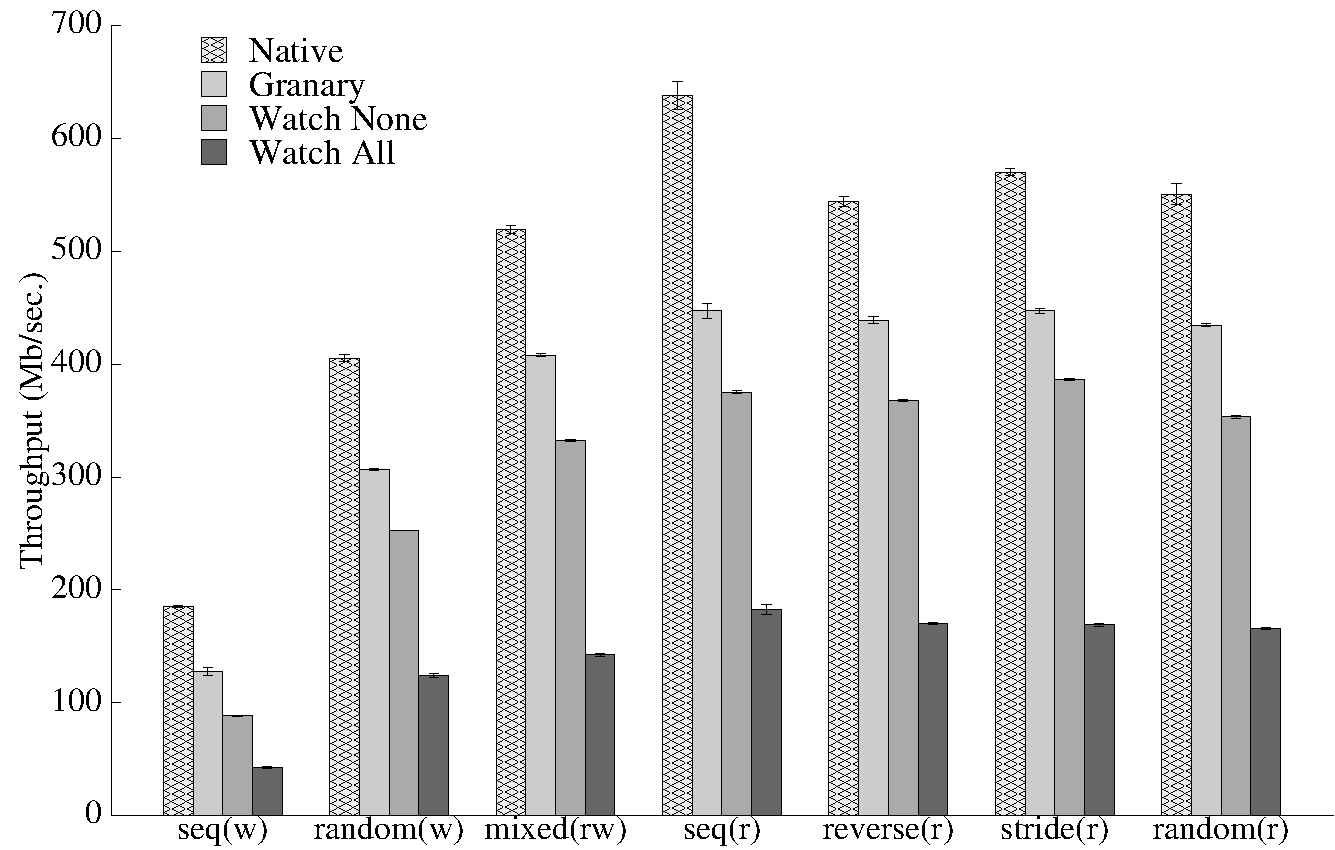
\includegraphics[width=4.5in]{thesis_code_driven.pdf}
\end{center}
\caption[Performance impact of code centric instrumentation.]{\label{fig:watchpoint_performance_code_driven}Throughput in MB/sec of common file system operations for code-centric instrumentation. Direct IO is enabled to bypass the effect of the OS buffer cache on read requests. It compares the overhead of the watchpoint framework with the performance overhead of Granary and with native system.}
\end{figure}

\subsection{Iozone filesystem benchmark}
We used the \emph{iozone}~\cite{citeulike:919086} file system benchmark to measure the overhead of behavioral watchpoints on the throughput of common file system operations. In our experimental setup, we used the \texttt{ext3} file system module that was mounted on a RAMDisk of size 1GB. We enabled direct IO to avoid the effect of buffer cache on file system. The \emph{iozone}, in throughput mode, created two processes (reader, writer) that perform the file I/O operations on a file of size 480Mb with a record size of 4Kb. The watchpoint framework wraps the two most commonly used memory allocators in \texttt{ext3} and \texttt{jbd}: \texttt{\_\_kmalloc} and \texttt{kmem\_cache\_alloc}, to add watchpoints on the allocated objects. We evaluated both the code-centric \& data-centric approaches using \emph{iozone} and compared their performance.


%----

%We evaluated both code-centric and data-centric approach using \emph{iozone} and compared their performance in terms of the number of active watchpoints. 
%In data-centric instrumentation approach the behavioral watchpoint does not uses wrappers for attaching and detaching Granary at the interface. The framework attaches on traps raised by dereferencing of watched addresses and it detaches at the end of basic block or when the function returns. In this case we wrap the allocators by hot-patching kernel text and add watchpoints only when the allocation happens by the module code. 

\begin{table*}
\begin{center}
\vspace{1em}
\begin{tabular}{|l|r|r|}
  \hline
  \multicolumn{3}{|c|}{Watchpoint statistics for the code-centric instrumentations}  \\ \hline
  \hline
  & Watch None & Watch All \\
  \hline
  Number of basic blocks & 2249 & 5495\\
  \hline
  Number of basic blocks with watched memory operations & 0 & 1208\\
  \hline
  Number of executed basic blocks & 238782485 &  825836778 \\
  \hline
  Number of dynamic memory operations & 568643857 & 1693113417 \\
  \hline
  Number of watched memory operations & 0 &199495293 \\
  \hline
  Number of kernel hardware traps & 0 & 12630779 \\
  \hline
\end{tabular}
\caption[Watchpoint statistics for code centric instrumentation. The watchpoints are added on all module allocated objects.]{\label{table:code-centric-watchpoint_stats} The statistics of the watchpoint framework for code-driven instrumentation when module allocated objects are watched. It also shows the effect of watched objects leaked to the kernel. The increase in the number of hardware traps causes an increase in the number of basic blocks and the number of executed basic blocks.}
\end{center}
\end{table*}

\paragraph{Code-centric instrumentation:}
The code-centric approach comprehensively instruments the module code and dynamically adds watchpoint instrumentation at every memory reference. This baseline watchpoint instrumentation causes overhead even when there are no added watchpoints. In the code-centric approach the module always runs under the control of Granary and executes code from the code-cache. It uses the kernel and module function wrappers for fast attaching and detaching at the interface. %This causes an extra overhead on any interactions between the kernel and the modules.

In the code-centric instrumentation, we first evaluated the overhead of watchpoint instrumentation and the cost of using Granary as the underlying DBT system. This is important to understand the baseline cost of using the watchpoint framework. 

\Figref{watchpoint_performance_code_driven} represents the overhead of code-centric instrumentation on the throughput of file I/O operations. The overhead of the watchpoint framework increases to {\texttildelow}70\% when all objects allocated by the module are watched. This is because many of these watched objects are shared and leak to the kernel. When these objects are dereferenced in the kernel, they cause hardware traps because Granary detaches itself at the kernel interface and the watchpoint instrumentation is no longer added to the memory references. These hardware traps are costly and reattach the watchpoint framework which then instruments the kernel code transitively.


\begin{table*}
\begin{center}
%\caption{Performance of macrobenchmark}
\begin{tabular}{ |l||r|r|r| }
\hline
\multicolumn{4}{ |c| }{Access pattern of module allocated objects} \\ \hline
\hline
Memory Allocator & Size & Module Accesses Count  & Kernel Accesses Count\\ \hline
\multirow{5}{*}{$\_\_kmalloc$} & 8 & 1233865 & 0 \\ \cline{2-4}
 & 50 & 720 & 288\\ \cline{2-4}
 & 51 & 648 & 240\\ \cline{2-4}
 & 59 & 792 & 528\\ \cline{2-4}
 & 4096 & 23452 & 0 \\ \hline
 \hline
 \multirow{7}{*}{$kmem\_cache\_alloc$} & 16 & 31533 & 0 \\ \cline{2-4}
 & 24 & 25019188 & 0\\ \cline{2-4}
 & 32 & 2348 & 0\\ \cline{2-4}
 & 64 & 2469028 & 3099\\ \cline{2-4}
 & 112 & 21404553 & 0 \\ \cline{2-4}
 & 192 & 19902520 & 4916028 \\ \cline{2-4}
 & 768 & 57760206 & 37373718 \\ \cline{2-4}
 & 1024 & 34865132 & 7940485 \\ \cline{2-4}
 & 8196 & 299 & 821648 \\ \hline
 \hline
 \multirow{1}{*}{$\_get\_free\_page$} & 4096 & 820273 & 2973 \\ \hline
\end{tabular}
\caption[Memory access pattern of module allocated objects.]{\label{table:access_pattern_shared_objects}The memory accesses patten of the module allocated objects. It represents the number of times an object is getting accessed by the module and the kernel code. The objects are classified based on its size and the memory allocator used for allocation. %The post analysis  shows that file system \texttt{inode} objects with memory size 768 are most accessed object by the kernel. A watchpoint on \texttt{inode} object will generate maximum number of hardware traps.
}
\end{center}
\end{table*}

\begin{table*}
\begin{center}
\vspace{1em}
\begin{tabular}{|l|r|r|}
  \hline
  \multicolumn{3}{|c|}{Watchpoint statistics for the code-centric instrumentations}  \\ \hline
  \hline
  & Watch none \texttt{inode} & Watch All \\
  \hline
  Number of basic blocks & 2874 & 5495\\
  \hline
  Number of basic blocks with watched memory operations & 732 & 1208\\
  \hline
  Number of executed basic blocks & 266083908 &  825836778 \\
  \hline
  Number of dynamic memory operations & 594195510 & 1693113417 \\
  \hline
  Number of watched memory operations & 92600064 &199495293 \\
  \hline
  Number of kernel hardware traps & 5285701 & 12630779 \\
  \hline
\end{tabular}
\caption[Watchpoint statistics for code centric instrumentation. The watchpoints are added on all the module allocated objects except file \texttt{inode}s.]{\label{table:code-centric-node-inode-watchpoint_stats} The watchpoint statistics of the framework for code-driven instrumentation when all objects allocated by the modules (except \texttt{inode}s) are watched.}
\end{center}
\end{table*}

Table~\ref{table:code-centric-watchpoint_stats} represents the number of hardware traps encountered and number of executed basic blocks for the code centric instrumentation. The additional increase in the number of basic blocks ({\texttildelow}2.5{\footnotesize$\times$}) and the number of executed basic blocks ({\texttildelow}3.5{\footnotesize$\times$}) comes due to the kernel code instrumentation on hardware traps. It also shows that the one out of every sixteen watched memory operations causes hardware traps.

For understanding the source of these hardware traps, we developed a tool using the watchpoint framework which tracks the accesses of module allocated objects. We typed these objects based on their size and the memory allocator used for its allocation. Table~\ref{table:access_pattern_shared_objects} shows the access pattern of the module allocated objects. The post processing analysis shows that file system \texttt{inode} objects with its size ``768'' gets accessed by the kernel maximum number of times and adding watchpoint on \texttt{inode} objects cause maximum number of hardware traps.

We verified this by removing watchpoints from all \texttt{inode} objects and running \emph{iozone} in throughput mode. \Figref{watchpoint_performance_code_driven_none_inode} shows that the overhead for \emph{Watch All} decreases by {\texttildelow}50\% and is close to the overhead of baseline instrumentation i.e, \emph{Watch None}. The small differences in the overhead of \emph{Watch All} and \emph{Watch None} are because there were still some shared objects which was getting watched and causing hardware traps. Table~\ref{table:code-centric-node-inode-watchpoint_stats} shows the details about such objects.


\begin{figure}[t]
\begin{center}
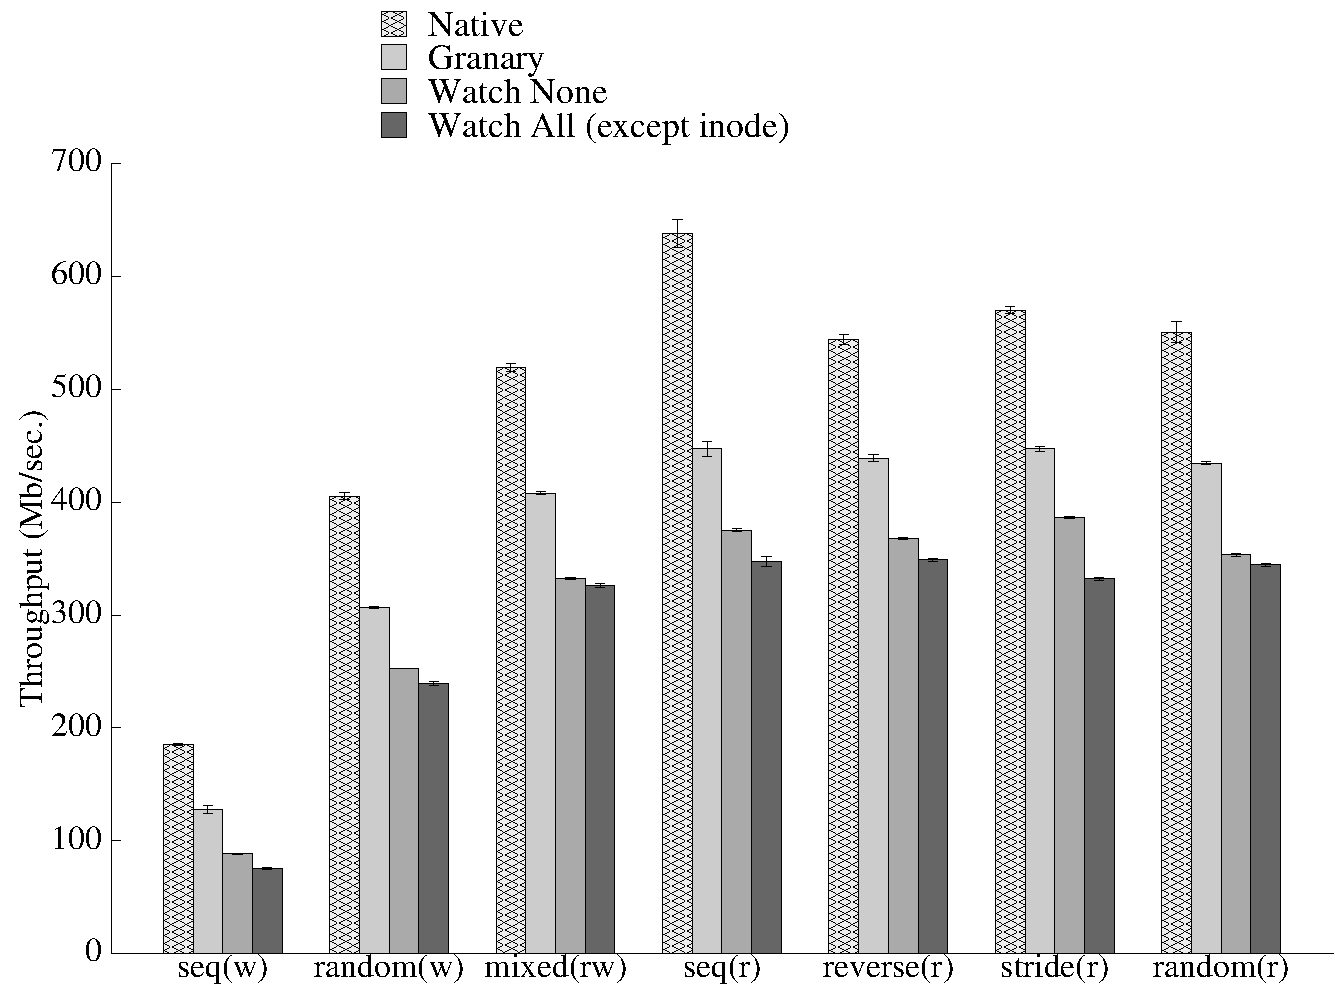
\includegraphics[width=4.5in]{thesis_code_none_inode.pdf}
\end{center}
\caption[Performance impact of code centric instrumentation. The watchpoints are added on all module allocated objects except file \texttt{inode}s.]{\label{fig:watchpoint_performance_code_driven_none_inode}Throughput in MB/sec of common file system operations for code-centric instrumentation when \texttt{inode} objects are not getting watched. The overhead of \emph{Watch All} decrease because of the less number of hardware traps and executed basic blocks.}
\end{figure}


The evaluation of code-centric instrumentation shows that the hardware traps on the kernel code are the major source of overhead in implementing behavioral watchpoints. These hardware traps can be removed by providing full kernel support to the code-centric instrumentation. Granary, being the underlying DBT-system, currently does not provide support for whole kernel instrumentation. 

%To understand the source of these hardware traps, we developed a tool using the watchpoint framework 


%We also studied the source of these hardware traps 


%The evaluation shows that a major contribution in the overhead of code-centric instrumentation comes due to Granary and its wrapping mechanism.

 %\Figref{watchpoint_performance_code_driven} shows the drop in throughput of filesystem operations when using the watchpoints instrumentation. As mentioned earlier \emph{watchpoint\_null} represents the overhead of baseline watchpoints instrumentation with no added watchpoints, and \emph{everything\_watched} shows the overhead where module-allocated objects are watched. We used code-centric instrumentation approach for the evaluation.

%In the previous section, we discussed that due to the limitations of Granary to instrument only the module code, our implementation of code-centric instrumentation is limited. We use code-centric instrumentation for executing the module code and data-centric instrumentation for the kernel code if the watchpoint leaks to the kernel. We also use three different policy for the code-centric instrumentation: transitive instrumentation policy, function-only instrumentation policy and basic-block instrumentation policy. The detail about these policies are discussed in section. Before evaluating the complete data-centric approach, we evaluated the compared the effect of three policies on code-centric instrumentation.



%\Figref{watchpoint_performance_code_driven} shows the overhead on the throughput of different filesystem operations. We also collected the watchpoint statistics for the the three policies. Table~\ref{table:data-centric-table} shows the number of hardware-exception encountered and the ration of executed basic block containing watched and unwatched addresses.

\begin{figure*}[t]
\begin{center}
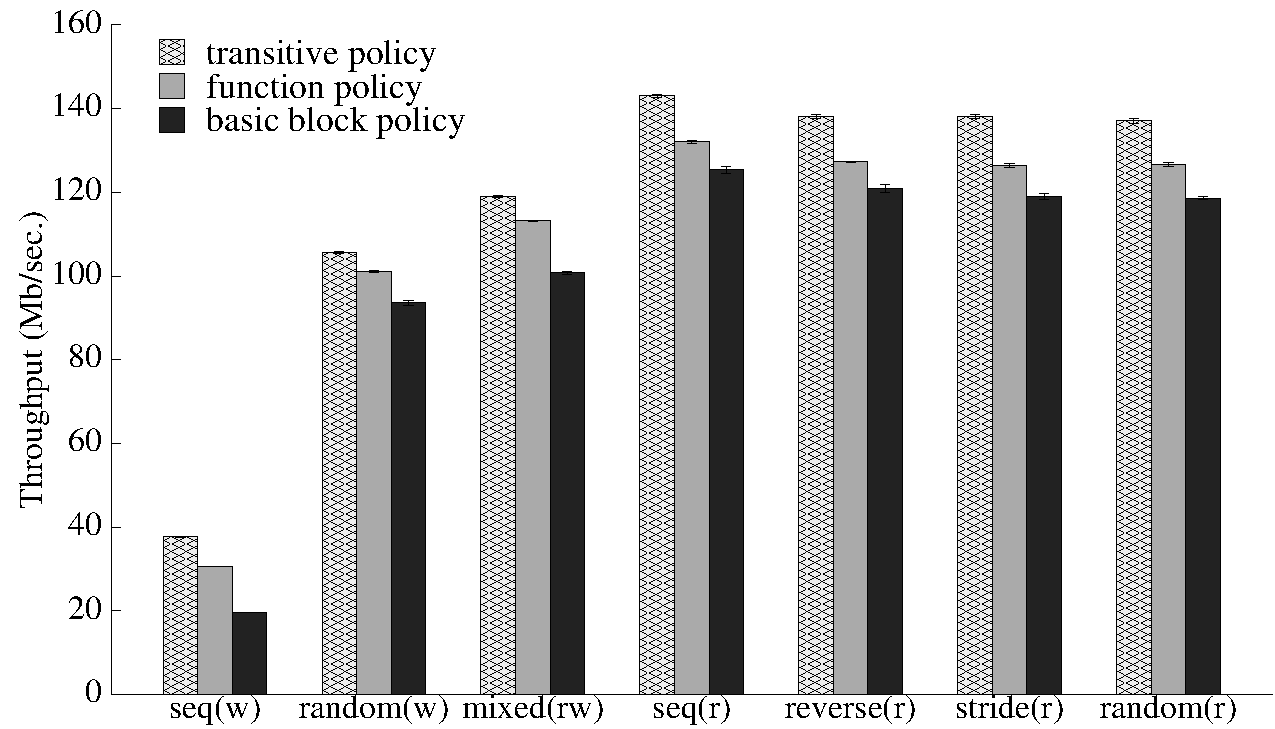
\includegraphics[width=4.5in]{thesis_data_driven.pdf}
\end{center}
\caption[Performance impact of data centric instrumentation.]{\label{fig:watchpoint_performance_data_driven}Throughput in MB/sec of common file system operations for data-centric instrumentation. It shows the overhead of three data-centric policies: transitive policy, function only, and basic block only policy.}
%for the watched address is shown.}
\end{figure*}


\paragraph{Data-centric instrumentation:}
We implemented data-centric instrumentation with three detach policies: i) transitive policy, ii) function-only policy and iii) basic block policy. Section~\ref{sec:data-centric} discusses each of the three policies in detail. %The data-centric instrumentation adds watchpoints on newly allocated objects through hot-patching and wrapping the kernel memory allocators. 


\begin{table*}
\begin{center}
\vspace{1em}
\begin{tabular}{|l|r|r|r|}
  \hline
  \multicolumn{4}{|c|}{Watchpoint statistics for data-centric instrumentation (with different detach policies)}  \\ \hline
  \hline
  & transitive & function & block \\
  \hline
  Number of basic blocks & 5755 & 3335 & 1144 \\
  \hline
  Number of basic blocks with watched memory operations & 1479 & 1218 & 1141\\
  \hline
  Number of executed basic blocks &  833167407  & 108965164 & 37378155\\
  \hline
  Number of dynamic memory operations & 1702295819 & 565666812 & 251985370\\
  \hline
  Number of watched memory operators & 336149753 & 234340514 & 206334774\\
  \hline
  Number of kernel hardware traps & 13403663 & 42259345 & 97518601\\
  \hline
  Number of module hardware traps & 112172 & 23496407 & 42902684\\
  \hline
\end{tabular}
\caption[Watchpoint statistics for data centric instrumentation.]{\label{table:data-centric-table} The statistics of the watchpoint framework for data-centric instrumentation when all the objects allocated by the modules are watched. It compares the three detach policies used by the data-centric approach.}
\end{center}
\end{table*}

We evaluated the overhead of data-centric instrumentation with \emph{iozone}, using the same experimental setup as with the code-centric instrumentations. We disabled the kernel and the module wrappers since they allow Granary to take complete control over the module code and prohibit the module code from running native. In data-centric instrumentation, the module code gets executed natively when there are no added watchpoints. 

Before comparing the code-centric and data-centric approaches, we first evaluated the three detach policies of data-centric instrumentation. \Figref{watchpoint_performance_data_driven} shows the overhead of each policy on the throughput of file I/O operations. The transitive policy instruments code aggressively and performs better than the function only and basic block detach policies. Table~\ref{table:data-centric-table} shows the number of executed basic blocks and the number of hardware traps encountered when each of the three detach policies are used. The transitive policy encounters the minimum number of hardware traps and executes the largest number of basic blocks. %The transitive policy also has large number of basic block with watched memory operations and this is because it adds more number of watchpoints on the newly allocated objects.

% executes the module code natively when no watchpoints get added and does not cause any runtime overhead in the system. It also uses three policies to reduce the cost of handling hardware traps. We first evaluated the three policies of data-centric instrumentation and compared their performance overhead along with the number of basic block executed and the hardware traps encountered by each of them. \Figref{watchpoint_performance_data_driven} shows the overhead of each policies on the throughput of file I/O operations for \texttt{ext3} module. The transitive policy has slight advantage over the function only and basic block policy because of the decrease in the number of hardware traps it needs to handle. There is also an increase in the number of basic block executed and this adds to the overhead of the transitive policy. Table~\ref{table:data-centric-table} shows how the number of executed basic blocks and the number of hardware traps encountered varies across the three policies. It also shows that the number of hardware traps encountered in module code is always less than the hardware traps at the kernel code. It represents that a majority of watched objects are shared and leaks to the kernel. These hardware traps also causes a significant overhead in the code-centric instrumentation and our approach of code-centric is more biased towards the data-centric.


\begin{figure}[t]
\begin{center}
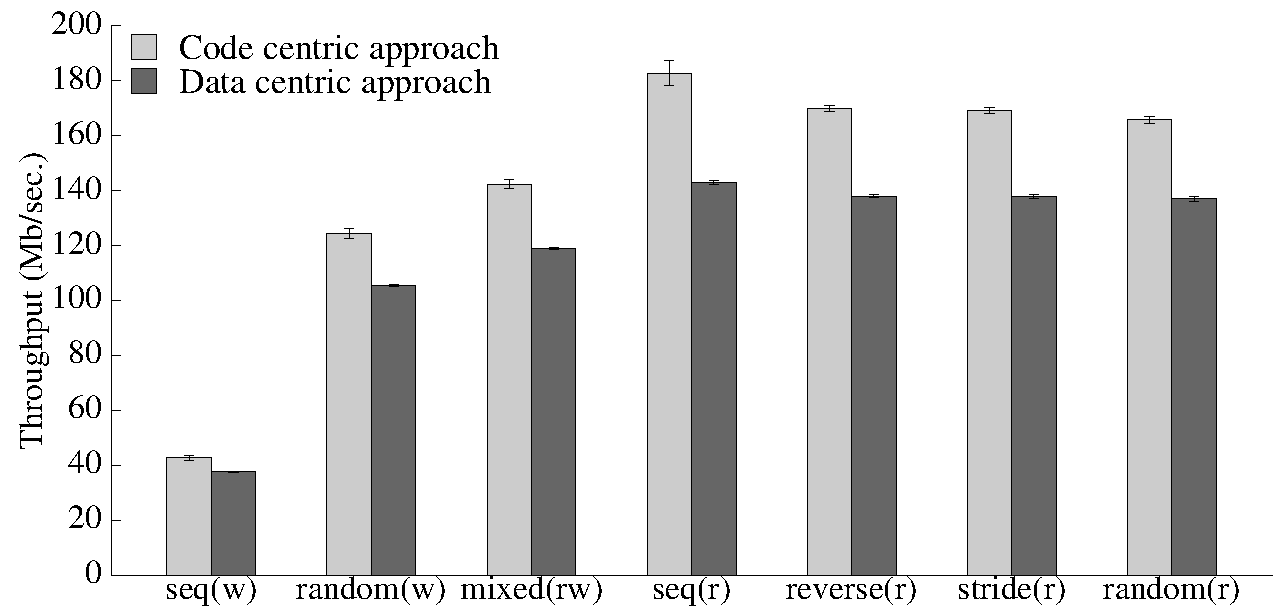
\includegraphics[width=6.0in]{thesis_data_code.pdf}
\end{center}
\caption[Performance impact of Data centric Vs Code centric instrumentation.]{\label{fig:watchpoint_performance}Throughput in MB/sec of common file system operations for the code-centric and data-centric approaches. The watchpoints are added on all objects allocated by the module.}
%for the watched address is shown.}
\end{figure}

%of the two reasons: i) the data-centric instrumentation handles more hardware traps which is costly, and ii) the number of watchpoints added in transitive detach policy is more than the code-centric instrumentations.

%In spite of increase in the number of hardware traps in the data-centric approach, it is performing better than the code-centric approach. This is because of the increase in the number of executed basic blocks. Also the code-centric approach suffers significantly due to the large number of hardware traps in the kernel code. The evaluation of three policies of data-centric approach also shows that the increase in the overhead due to hardware traps is getting compensated with the less number of basic block being executed. Table~\ref{table:data-centric-table} shows that the number of hardware traps encountered in transitive policy is 5x less than the basic block policy but it is executing 10x more basic block and thus not getting much advantages in terms of performance. The code centric approach is also using the kernel and the module wrappers which has an additional cost.

\begin{figure}[!h]
\begin{center}
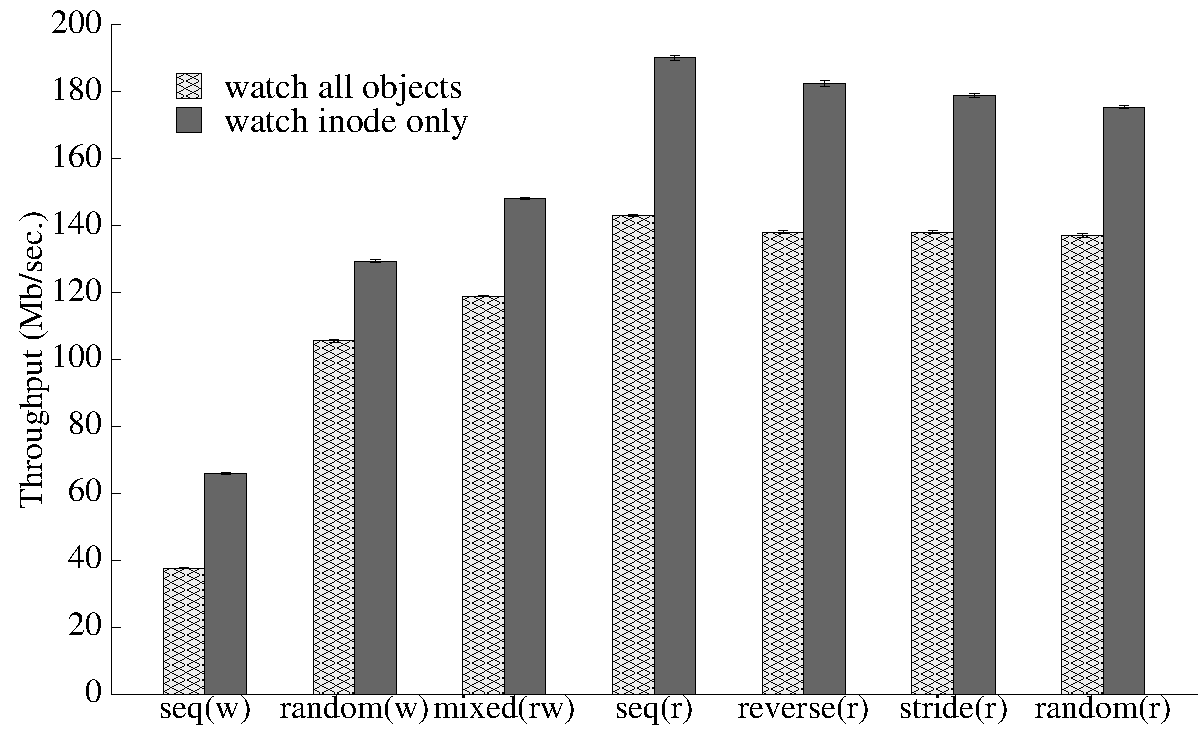
\includegraphics[width=6.0in]{thesis_watch_inode.pdf}
\end{center}
%\end{figure}

%\begin{figure}
\begin{center}
\vspace{1em}
\begin{tabular}{|l|r|r|}
  \hline
  \multicolumn{3}{|c|}{Watchpoint statistics for selective instrumentation in data centric instrumentation }  \\ \hline
  \hline
  & Watch \texttt{inode}s & Watch all \\
  \hline
  Number of basic blocks & 4217 & 5755\\
 % \hline
  Number of basic blocks with watched memory operations & 562 & 1479 \\
  \hline
  Number of executed basic blocks &  735367411 &  833167407 \\
  \hline
  Number of dynamic memory operations & 1519057148 & 1702295819 \\
  \hline
  Number of watched memory operators & 87433900 & 336149753 \\
  \hline
  Number of kernel hardware traps & 5522314 &  13403663 \\
  \hline
  Number of module hardware traps & 11234 & 112172 \\
  \hline
\end{tabular}
%\caption{\label{fig:watchpoint_inode_compare} Throughput in MB/sec of common file system operations and the watchpoint statistics when watchpoints are added selectively and only on \texttt{inode} objects.}
\caption[Performance impact of selective instrumentations for data-centric approach.]{\label{fig:watchpoint_inode}Throughput in MB/sec of common file system operations and the watchpoint statistics for data-centric instrumentation when watchpoints are added selectively and only for \texttt{inode} objects. The evaluation is done for transitive detach policy.}
%for the watched address is shown.}
\end{center}
\end{figure}


\Figref{watchpoint_performance} compares the overhead of code centric and data centric instrumentation. It shows that the code centric instrumentation performs better than the data centric instrumentation when all objects allocated by the module are watched. This is because the code centric instrumentation handles less hardware traps, which is costly and affects the performance of the system. Our evaluation compares the code centric instrumentation with the data centric instrumentation using transitive detach policy.


\begin{figure}[!h]
\begin{center}
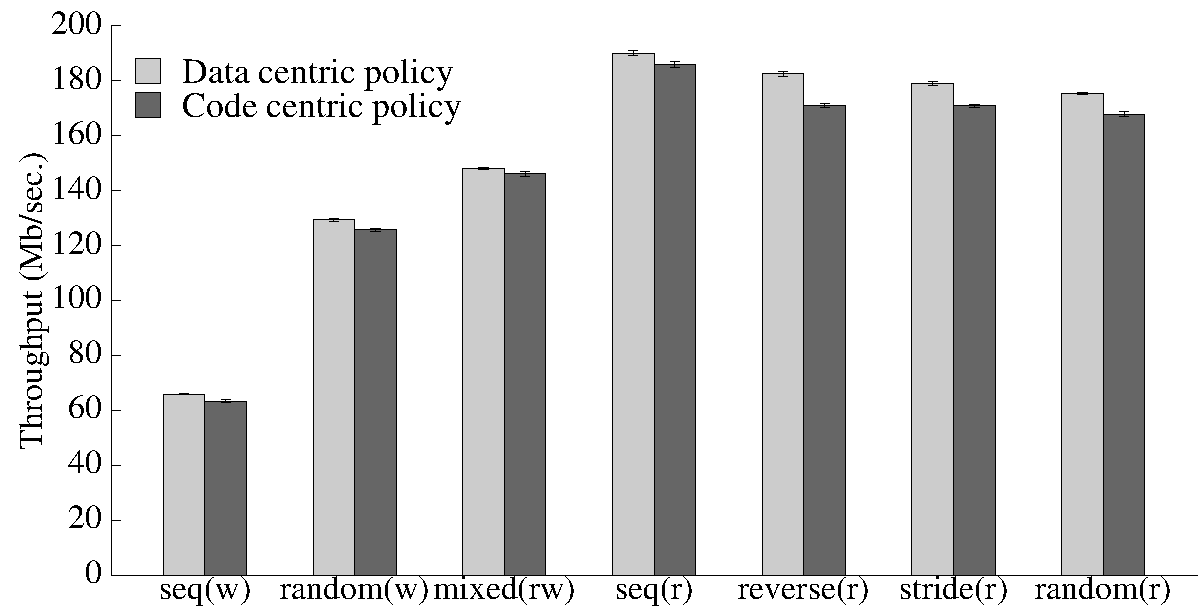
\includegraphics[width=6.0in]{thesis_watch_inode_compare.pdf}
\end{center}
%\caption{\label{fig:watchpoint_inode_compare}Throughput in MB/sec of common file system operations when watchpoints are added selectively and only for \texttt{inode} objects. The evaluation is done with transitive instrumentation policy.}
%for the watched address is shown.}
%\end{figure}  

%\begin{table*}
\begin{center}
\vspace{1em}
\begin{tabular}{|l|r|r|}
  \hline
  \multicolumn{3}{|c|}{Watchpoint statistics for selective instrumentation (watch \texttt{inode} objects)}  \\ \hline
  \hline
  & Code centric & Data centric \\
  \hline
  Number of basic blocks & 5405 & 4217 \\
 % \hline
  %Number of basic blocks with watched memory operations & 563 & 563 \\
  \hline
  Number of executed basic blocks &  814496751  & 735367411 \\
  \hline
  Number of dynamic memory operations & 1684738365 & 1519057148\\
  \hline
  Number of watched memory operators & 91699675 & 87433900 \\
  \hline
  Number of kernel hardware traps & 5446745 & 5522314 \\
  \hline
  Number of module hardware traps & 0 & 11234 \\
  \hline
\end{tabular}
\caption[Performance impact of selective instrumentations. The watchpoints are added on all file \texttt{inode} objects.]{\label{fig:watchpoint_inode_compare} Throughput in MB/sec of common file system operations and the watchpoint statistics when watchpoints are added selectively and only on \texttt{inode} objects.}
\end{center}
%\end{table*}
\end{figure}



\begin{figure}[!h]
\begin{center}
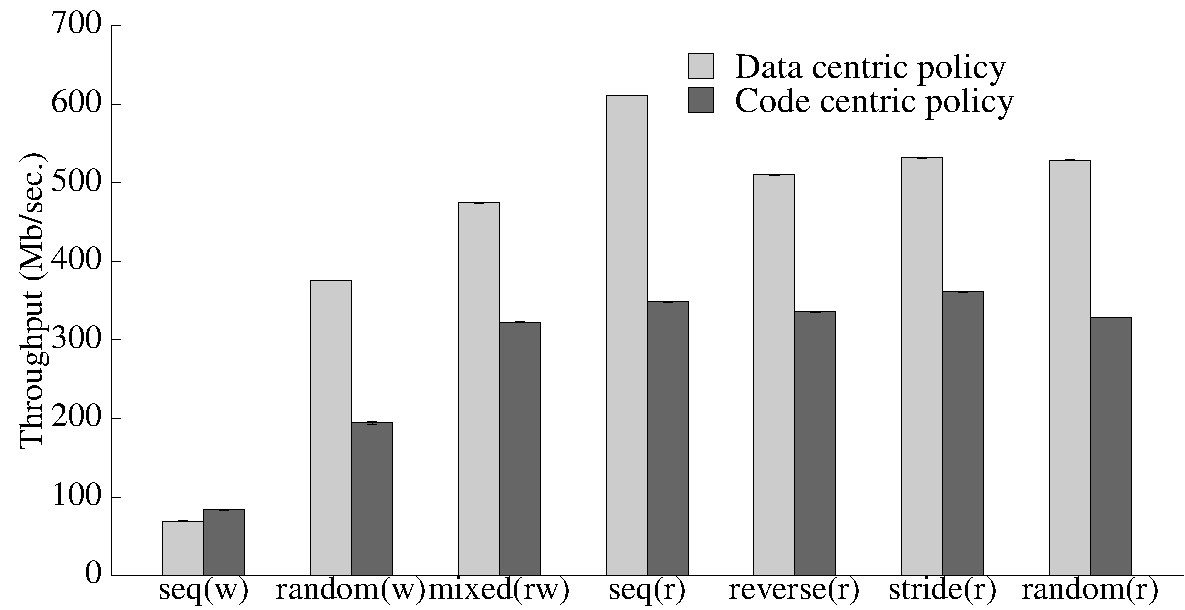
\includegraphics[width=6.0in]{thesis_selective_watch_no_inode.pdf}
\end{center}
\vspace{1em}
\begin{center}
\begin{tabular}{|l|r|r|}
  \hline
  \multicolumn{3}{|c|}{Watchpoint statistics for selective instrumentation (no hardware traps on kernel code)}  \\ \hline
  \hline
  & Code centric & Data centric \\
  \hline
  Number of basic blocks & 2259 & 1171 \\
  \hline
  Number of basic blocks with watched memory operations & 179 & 189 \\
  \hline
  Number of executed basic blocks &  238740476  & 105345884 \\
  \hline
  Number of dynamic memory operations & 568556578 & 221904835\\
  \hline
  Number of watched memory operators & 45649624 & 45637811\\
  \hline
  Number of module hardware traps & 0 & 10244480 \\
  \hline
\end{tabular}
\caption[Performance impact of selective instrumentations. The watchpoints are added on objects that are not getting accessed by the kernel code]{\label{fig:watchpoint_none_inode_compare} Throughput in MB/sec of common file I/O operations and the statistics of the watchpoint framework when watchpoints are added to the objects selectively which are not getting accessed by the kernel. This removes the effect of hardware traps from the code-centric instrumentations.}
\end{center}
%\end{table*}
\end{figure}
%on the throughput of file operations when only inode gets watched. In this case we used transitive policy for the evaluation.  

\paragraph{Selective instrumentation:}
The data centric approach enables selective instrumentation by adding watchpoints on selected objects. We first evaluated the performance of selective instrumentation by adding watchpoints only on file \texttt{inode} objects. \Figref{watchpoint_inode} shows the overhead of selective instrumentation and compares it with the overhead of data-centric instrumentation when all the module allocated objects are watched. Selective instrumentation performs better since it adds less watchpoints thus encountering fewer hardware traps, and executing fewer instrumented basic blocks.

We also compared the performance of selective instrumentation when using code-centric and data-centric approaches. \Figref{watchpoint_inode_compare} compares the overhead of selective instrumentation for both the approaches. It shows that selective instrumentation using data centric instrumentation has less overhead than with code centric instrumentation. This is because fewer basic blocks gets executed with data-centric instrumentation. The number of hardware traps encountered in both the approaches are also approximately same, causing similar overhead. 


The evaluation of code-centric approach shows that a major source of overhead in code-centric instrumentation comes due to adding watchpoints on file \texttt{inode} objects. These objects gets accessed mostly by the kernel code causing hardware traps. We removed the effect of these hardware traps from code-centric instrumentation by adding watchpoints selectively on the objects accessed only by the modules. We took the help of table~\ref{table:access_pattern_shared_objects} for adding watchpoints on the objects selectively.

 \Figref{watchpoint_none_inode_compare} represents the overhead of selective instrumentations for data-centric approach and compares it with the code-centric instrumentation. It shows that the selective instrumentation reduces the overhead of using the watchpoint framework to {\texttildelow}5\% where as the baseline instrumentation for code-centric approach causes an overhead of {\texttildelow}40\%. This is because the selective instrumentation executes less number of basic blocks ({\texttildelow}2.3{\footnotesize$\times$}). The evaluation also shows that the performance of sequential write operation in case of data-centric approach is less than the code-centric. We analyzed the behavioral of write operations and found that {\texttildelow}50\% of the total hardware traps was only happening during sequential write operations. This could be a reason of sequential write not performing better.    

 The evaluation of both, the code-centric and data-centric approaches for implementing behavioral watchpoints, shows an interesting trade-off between the amount of instrumented code executed from the code-cache and how much of that code actually needs to be instrumented. The code-centric approach always suffers from the overhead of baseline instrumentation since it always executes instrumented basic block from code cache. The data-centric instrumentation overcome this by adding instrumentation on-demand. However, it suffers from the high cost of the hardware traps which triggers the instrumentation. The number of executed basic blocks also increases with the hardware traps which causes additional overhead.

 We also saw that the number of hardware traps depend on the type of the watched objects. Adding watchpoints on frequently accessed shared objects such as file \texttt{inode}s, causes a large number of traps affecting the performance of the watchpoint framework where as watching relatively less accessed objects such as \texttt{ext3\_block\_alloc\_info} causes less traps improving the performance of the data-centric instrumentation.

 The advantages and disadvantaged of both the approaches opens up the space to further explore the possibility of switching between the two approaches at runtime. This will reduce both the overhead of baseline instrumentation and the cost of hardware traps, thus improving the performance of the system. The evaluation of code-centric instrumentation also shows its need to provide the whole kernel instrumentation support. We plan to take this as an immediate future work.

 %The evaluation of the watchpoint framework using \emph{iozone} shows the


 %It shows that the selective instrumentation using data-centric approach reduces the overhead of using the watchpoint framework 


 %for both the code-centric and data-centric approaches.



 %by adding watchpoints on such objects. The data centric instrumentation in such case performs much better than the code centric approach and the performance of data centric instrumentation is close to that of the native system. 


%and added watchpoints selectively on objects which does not get accessed by the kernel.


%, we saw that a major source of overhead in code centric approach is the number of hardware traps. Much of these hardware traps occur due to adding watchpoints on \texttt{inode} objects and the code centric instrumentation was performing worse when it was getting watched. To remove the effect of hardware traps in selective instrumentation, we took the help of table~\ref{table:access_pattern_shared_objects} and added watchpoints selectively on objects which does not get accessed by the kernel. \Figref{watchpoint_none_inode_compare} compares the overhead of selective instrumentations by adding watchpoints on such objects. The data centric instrumentation in such case performs much better than the code centric approach and the performance of data centric instrumentation is close to that of the native system. 

%the number of instrumented basic block executed in case of data-centric approach is less than the code-centric approach. 
%However, it also shows that there are more hardware traps encountered with data-centric approach.

%The watchpoint gets added to the objects selectively. We evaluated the performance of selective instrumentation by adding watchpoints only to the \texttt{inode}s. \Figref{watchpoint_inode} compares the overhead on the throughput of file operations when only inode gets watched. In this case we used transitive policy for the evaluation.   
% the overhead of code-centric and data-centric approach 

%using complete data-centric approach.



%from providing the complete data-centric approach by wrapping all the function pointers at the interface for faster attach and detach.

%and we also used the same experimental setup for running the benchmark. We also disabled the wrappers for fast attach and detach since it prohibits the framework from providing the complete data-centric approach by wrapping all the function pointers at the interface for faster attach and detach.


%\subsection{Filebench}
%We evaluated the real workload using Filebench file system benchmark.

\subsection{Macrobenchmark}
We further evaluated the overhead of the behavioral watchpoint framework using a file system macrobenchmark consisting common system utilities. We used the same experimental setup and mounted the \texttt{ext3} module on a RAMDisk of size 1GB. The macrobenchmark operated on the Linux source tree (\texttt{linux-3.2.50}). Table~\ref{table:system_utils-benchmark} shows the overhead of behavioral watchpoints on the standard system utilities. For both the code-centric and data-centric approaches, the framework adds watchpoints selectively on all \texttt{inode} objects allocated from the look-aside buffer. The evaluation shows data-centric instrumentation is performing better than code-centric instrumentation when used for watching objects selectively all the \texttt{inode} objects.


\begin{table*}
\begin{center}
\vspace{1em}
\begin{tabular}{|l|r|r|r|}
  \hline
   & Native execution & Data centric approach & Code centric approach \\
  \hline
  cp & 6.64 & 10.82 & 11.61\\
  \hline
  tar & 2.64 & 3.84 & 4.16\\
  \hline
  stat & 3.90 & 5.12 & 5.44\\
  \hline
  grep & 3.94 & 5.36 & 5.54\\
  \hline
\end{tabular}
\caption[Performance impact of the watchpoint framework on macrobenchmark]{\label{table:system_utils-benchmark}The CPU (system \& user) time for the standard system utilities performing file system operations on a RAMDisk of size 1GB. The framework adds watchpoints selectively on all \texttt{inode} objects of the \texttt{ext3} module.}
\end{center}
\end{table*}


\begin{figure*}[t!]
\begin{multicols}{2}
\begin{center}
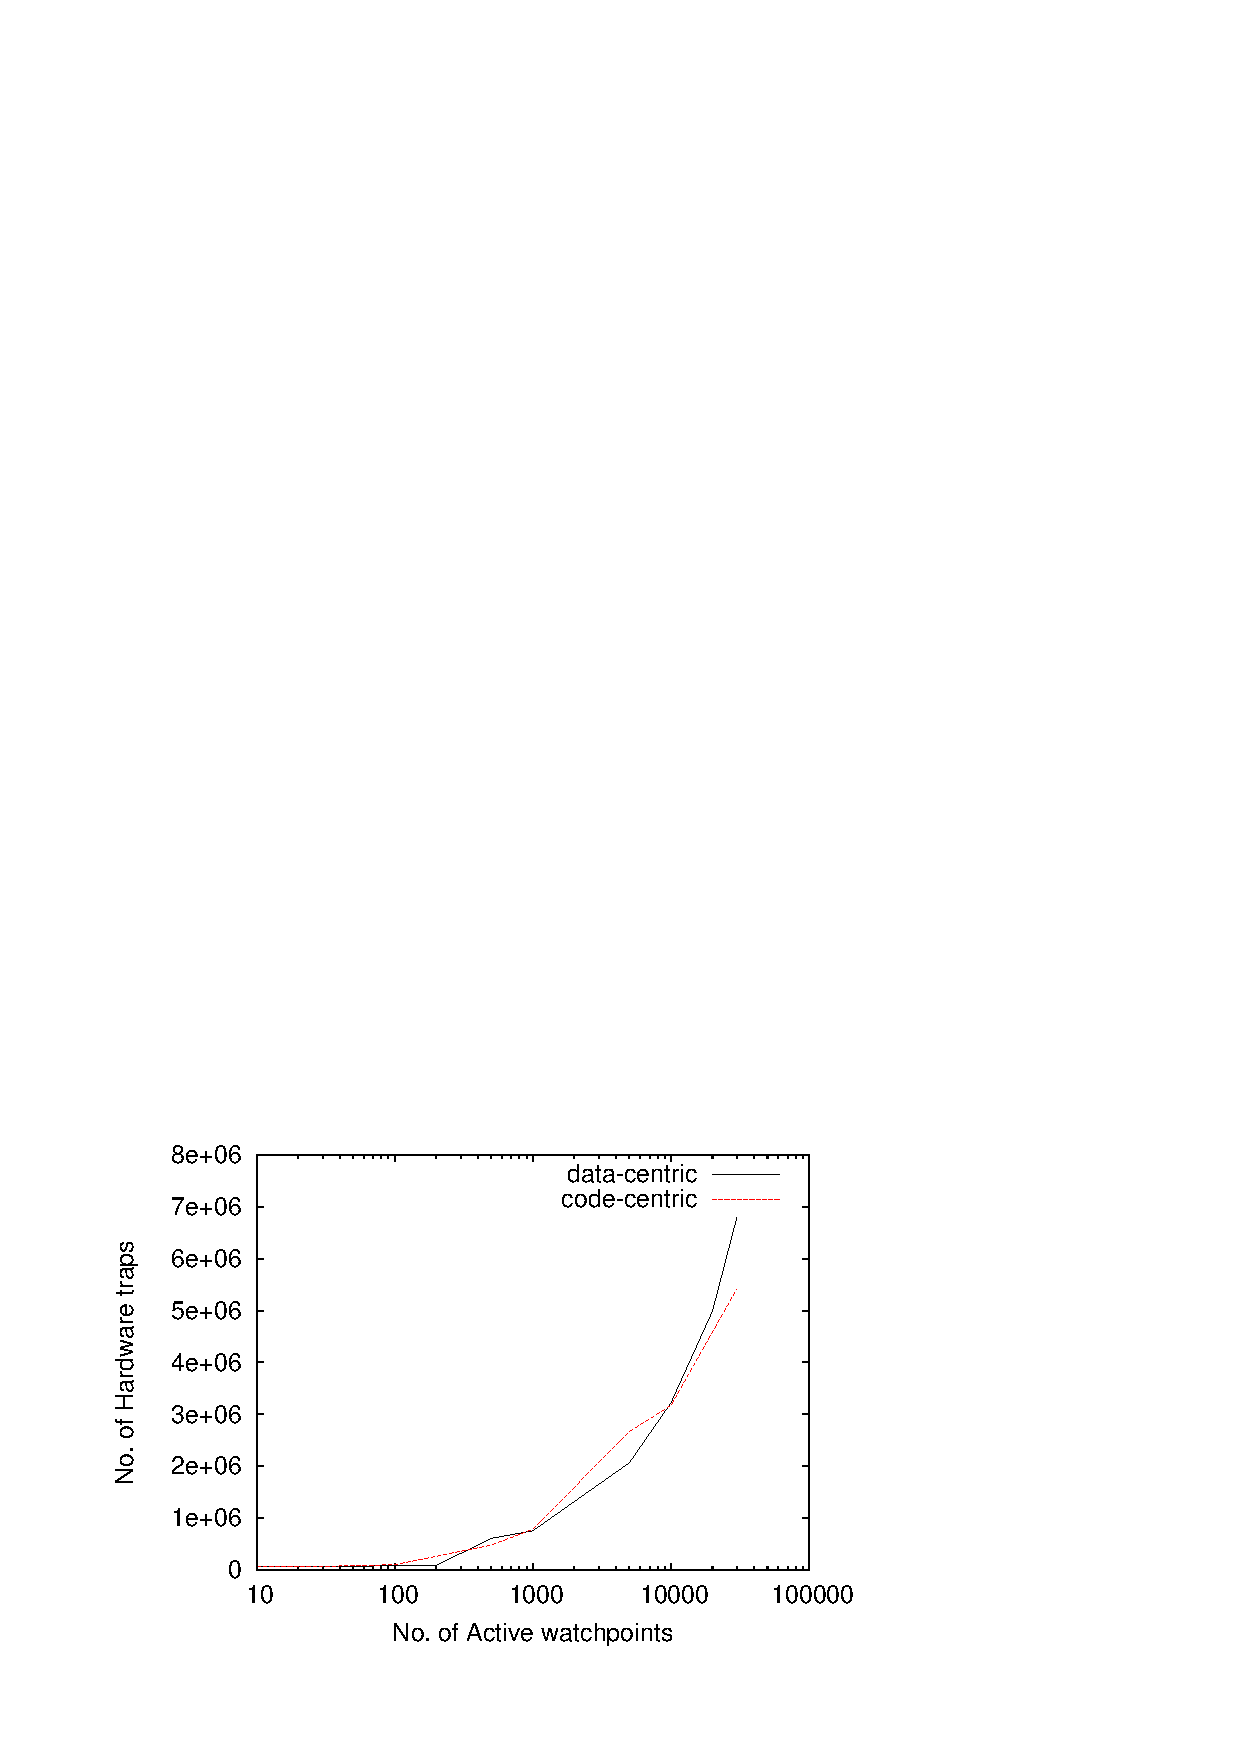
\includegraphics[width=3.5in]{hardware_traps.pdf}
\end{center}
\columnbreak
\begin{center}
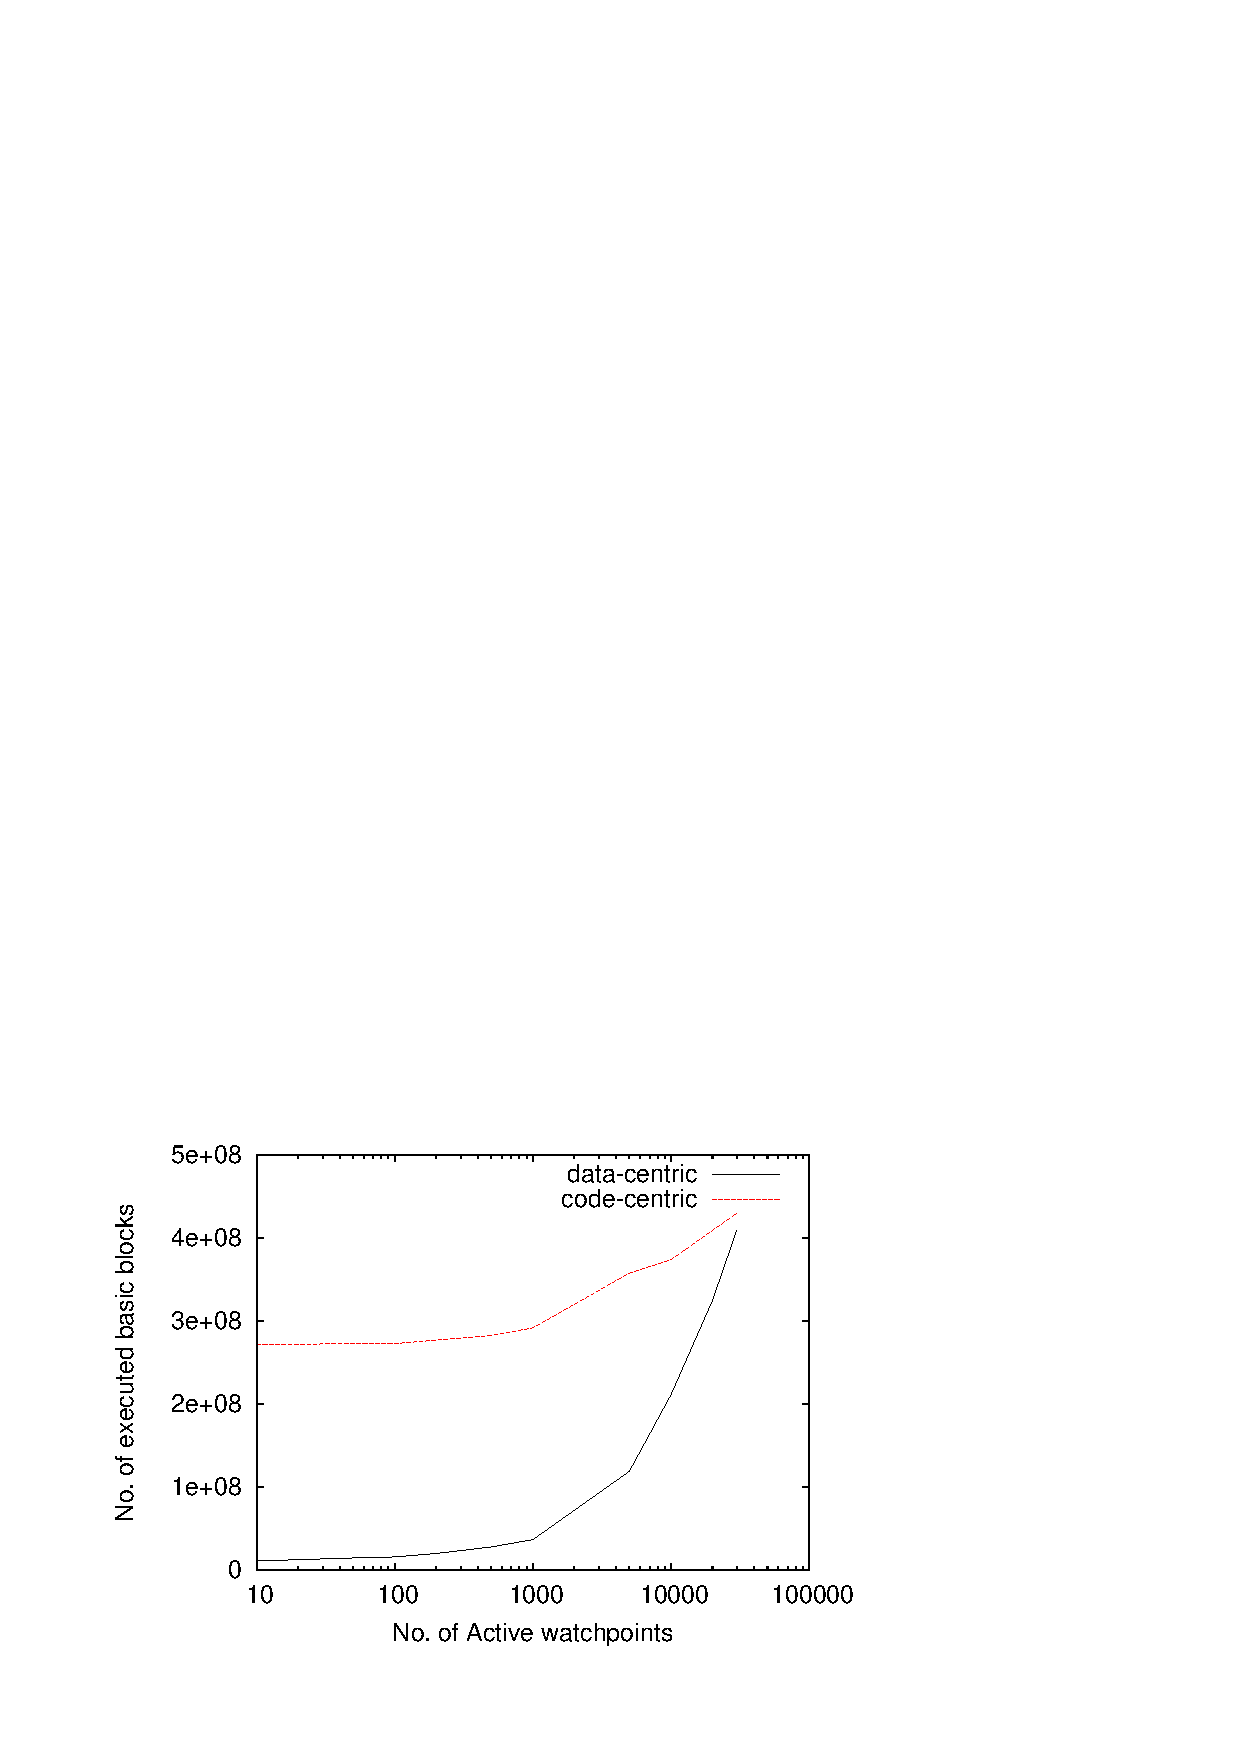
\includegraphics[width=3.5in]{executed_bb_data.pdf}
\end{center}
\end{multicols}
\caption[Cost profile of the watchpoint framework in terms of number of added watchpoints.]{\label{fig:traps_profile}The changes in the number of hardware traps and the number of executed basic blocks with the changes in number of added watchpoints.}
\end{figure*}

In both the code-centric and data centric approaches, the major factors which affects the performance are the number of basic block executed and the number of hardware traps encountered during the execution. We also used microbenchmark to study the changes in the number of hardware traps and the basic block executed with the change in the number of watchpoints. \Figref{traps_profile} shows that both the code centric instrumentation and data centric instrumentation encounters same number of hardware traps. This is because we add watchpoints selectively on all \texttt{inode} objects which gets accessed both by the module and the kernel code equally causing hardware traps. We also see fewer occurrences where the number of traps in case of data centric is less than the code centric instrumentation. One reason for this could be that the code centric instrumentation always detaches itself at the interface where as the data centric instrumentation, with transitive detach policy, does not always detaches itself at the interface.

\Figref{traps_profile} also shows that with fewer watchpoints the code centric instrumentation still executes many more basic blocks than the data centric approach. This causes increased overhead for code centric instrumentation even when fewer watchpoints are added. 




% and causes more overhead even when the 


% We also discussed previously that data centric instrumentation is useful when watchpoints are added on objects 

\begin{table*}
\begin{center}
\vspace{1em}
\begin{tabular}{|l|l|l|}
  \hline
   Workload & Setting & Data Size \\
  \hline
  Fileserver & nfiles=10K & 1.2GB \\
  \hline
  Webserver & nfiles=1K, & 14.76MB \\
  \hline
  Webproxy & nfiles=10K & 154MB \\
  \hline
  Varmail & nfiles=1K & 14.76MB \\
  \hline
\end{tabular}
\caption[Filebench server benchmark workload characteristics.]{\label{table:filebench-benchmark}Benchmark characteristics.}
\end{center}
\end{table*}


\begin{figure}[!h]
\begin{center}
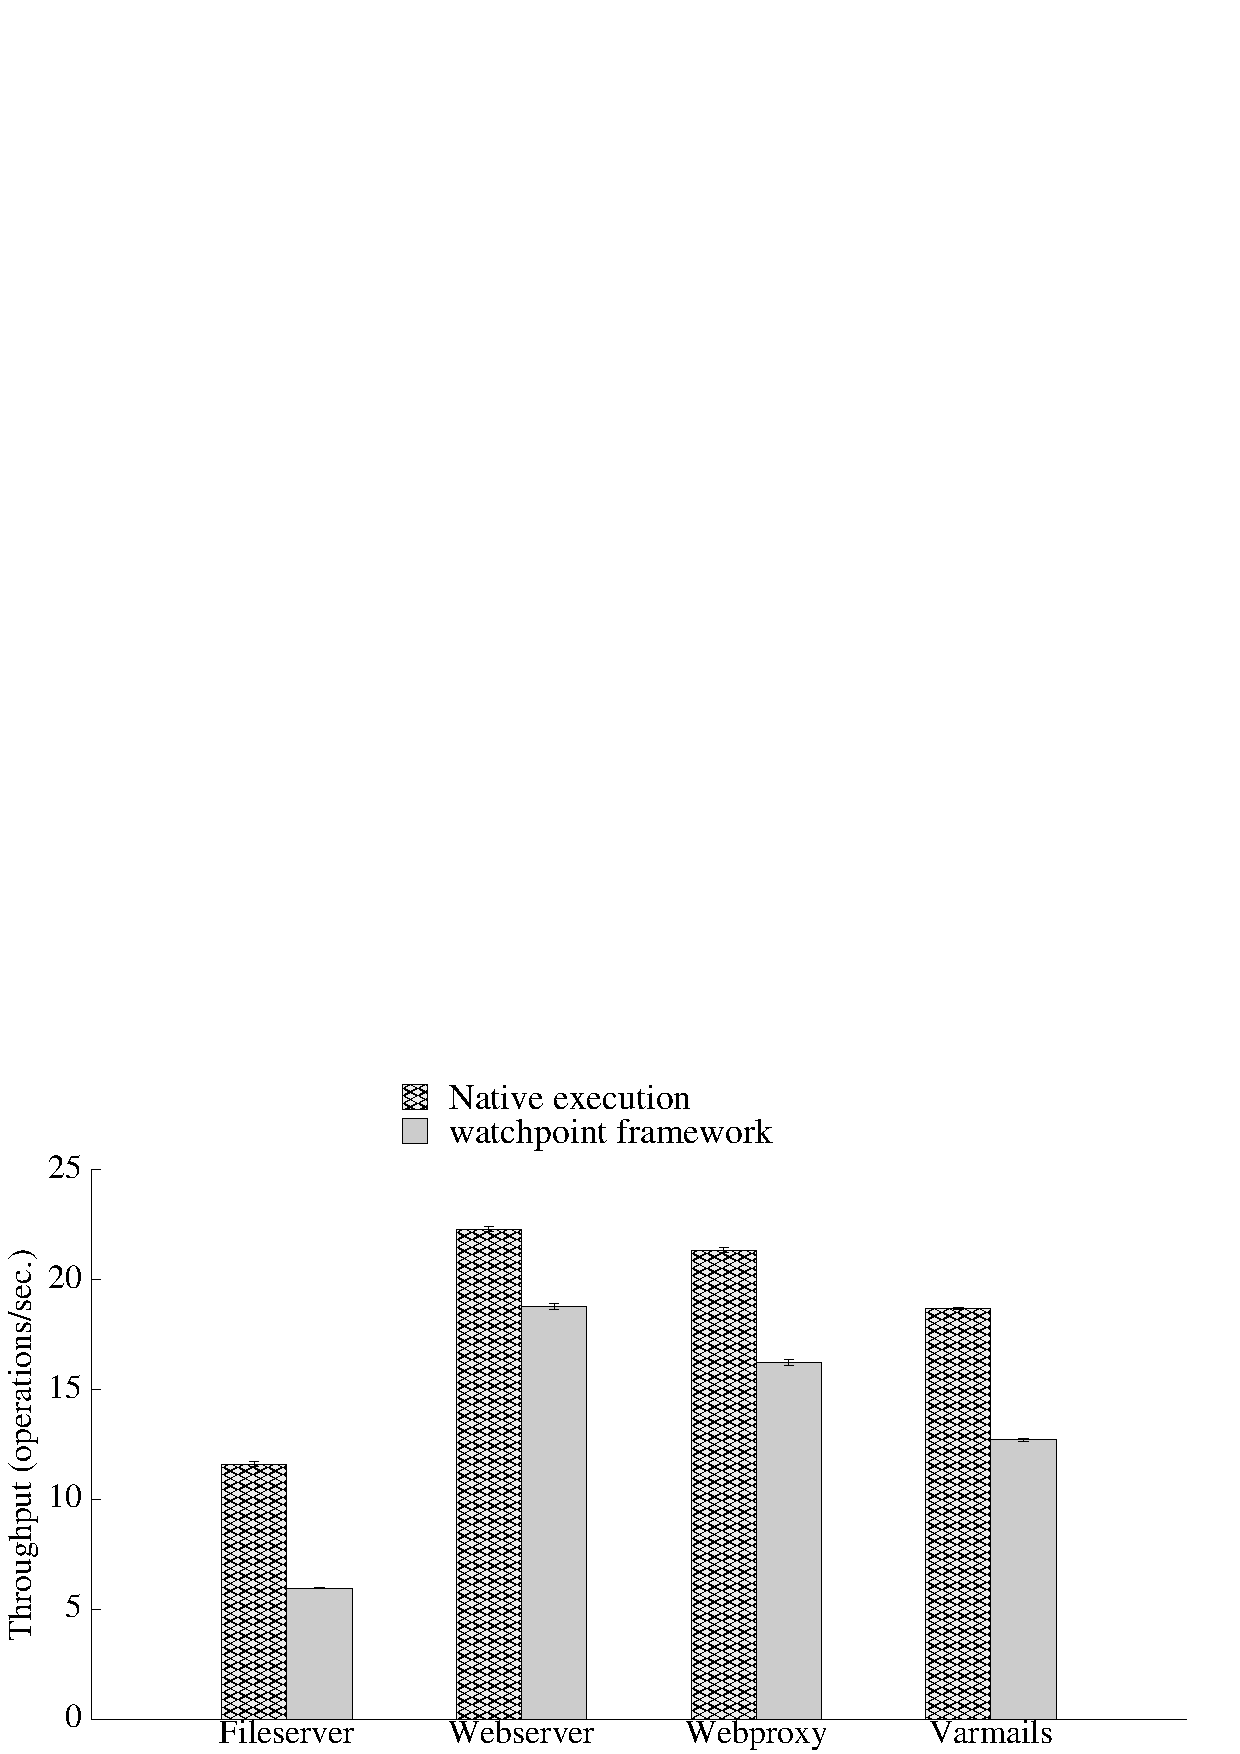
\includegraphics[width=6.0in]{filebench.pdf}
\end{center}
\caption[Performance impact of the watchpoint framework on Filebench server benchmark workloads.]{\label{fig:sever_performance}Throughput in file system operations/sec for the filebench workload personalities shown in Table~\ref{table:filebench-benchmark}.}
%for the watched address is shown.}
\end{figure}




\subsection{Server Benchmark}
We used the Linux port of Filebench version 1.4.9, with four of the standard server workload personalities, to evaluate the watchpoint framework. We used the same experimental setup as with the \emph{iozone} and enabled default settings to define the workload characteristics. The relevant characteristics for the workloads are shown in Table~\ref{table:filebench-benchmark}. With the default characteristics, the datasets easily fit in the RAMDisk used for evaluation. This does not limit the workload with the performance of I/O operations.

\Figref{sever_performance} shows the throughput of the different Filebench server workloads. For evaluation we used data-centric instrumentation with all file \texttt{inode} objects getting watched. The data centric instrumentation reduces the throughput for all the workload personalities by ~40\%. We also evaluated the code-centric instrumentation using Filebench and noticed similar drop in the throughput but we are not showing it here.

%Null Client reduces
%throughput by 3X for fileserver, and by 4.5X and 4.2X for webserver
%and webproxy, respectively. There is only a small additional
%reduction in throughput with Instruction Count. We can see that
%the drop in throughput is correlated with the number of threads
%used in the workload, with webserver and webproxy both using
%100 threads. The overhead for varmail, which syncs its data to disk
%frequently, is much lower, with only a 1.4X drop in throughput.

%We also evaluated the performance of behavioral watchpoints using real workloads. We mounted \texttt{ext3} file system module on a disk of size 20GB and used Filebench to simulate the real workloads. Table~\ref{table:filebench-benchmark} shows the characteristics of the workload we used for the evaluation.


%We used same experimental setup and mounted \texttt{ext3} module on RAMDisk of size 1GB. The macrobenchmark operated on the source tree of \texttt{linux-3.2.50} branch. We used the following five benchmarks to evaluate the performance overhead of the watchpoint framework: 

%\begin{enumerate}
%	\item \emph{MakeDir:} It reads the directories subtree of source program and constructs the identical target directories subtree. It uses \texttt{mkdir} utility for creating the directories recursively.
%	\item \emph{Copy:} It copies all the files from source files subtree to the target files subtree. We used \texttt{rsync} command to copy the files from the source directory to the target directory.
%	\item \emph{ScanDir:} It recursively goes to all the files in target directory and performs the stat operation on each file.
%	\item \emph{ReadAll:} It reads every byte of the every file in the target directory.
%	\item \emph{Compile:} It compiles and links all the files for the source program.
%\end{enumerate}


%Behavioral watchpoints uses non-canonical address to add watchpoints with the allocated objects. This provides the opportunity to implement data-centric instrumentation. Data-centric instrumentation is particularly important when watchpoints are unlikely to be triggered. We implemented three different policy for data-centric instrumentation: i) transitive policy, ii) function-only policy and iii) basic block policy. The details about it is provided in section. 

%Data-centric instrumentation also uses three different instrumentation policies and the details of which is provided in section.
%We used \emph{iozone} to evaluate the performance of data-centric instrumentation and we also used the same experimental setup for running the benchmark. We also disabled the wrappers for fast attach and detach since it prohibits the framework from providing the complete data-centric approach by wrapping all the function pointers at the interface for faster attach and detach.

%In this experiment, We studied the effect of hardware exceptions and watchpoint instrumentation overhead on the performance of filesystem throughput. We used the three data-centric policies for the evaluation and compared their performance in terms of the number of hardware exception encountered and the number of instrumented basic block executed. 

%Figure~\ref{fig:watchpoint_performance_data_driven} shows the throughput of common filesystem operations for data-centric instrumentation approach. Table~\ref{table:data-centric-table} shows the number of traps encountered along with the number of executed basic block and number of memory operations performed. The evaluation result shows the performance decrease with the number of traps but it gets compensated by executing less number of basic blocks and performing less number of memory operation which has an additional cost of watchpoint instrumentation.

% We also evaluated the number of hardware exception encountered and the number of basic block executed for each policies.



 %We also varies the number of watchpoints to see how the cost of data-centric instrumentation varies with the number of added watchpoints.


%These allocated objects when gets accessed causes hardware exceptions or traps. Behavioral watchpoint framework uses this to implement watchpoint instrumentation on trap. This approach allows selective instrumentation and can take advantage of low overhead when watchpoints are unlikely to be triggered. The trap-based instrumentation approach uses three different instrumentation policy: policy 1 includes the transitive instrumentation where the framework attaches itself on trap and instruments till it finds the indirect call or return and detaches itself. Policy 2 instruments the body of the function which encounters the trap and changes policy to go native on call and return. Policy 3 is the most conservative policy and tries to instruments minimum of the code. The instrumentation framework attaches itself on trap and detaches and goes to native execution on any control transfer, instrumenting only single basic block at a time. We evaluated all the three instrumentation policy by running the \emph{Iozone}~\cite{citeulike:919086} and studying the throughput of common file system operations. In trap-based instrumentation approach behavioral watchpoint is implemented on trap. We also used microbenchmark to evaluate the cost of taking trap and studied how the number of these traps increases over different policy and affects the performance.







%One of the important feature of data-driven instrumentation is the ability to watch objects selectively. The selective addition of watchpoints will have less instrumentation cost and also the number of hardware exception encountered will be less. We evaluated the performance of selective instrumentation by adding watchpoints to only \texttt{inode} objects. Figure~\ref{fig:watchpoint_inode} the overhead when only inode gets watched and compares it with everything watched. However the selective instrumentation of objects may suffer from the cold code-cache effect and it can cause high overhead.


%We also studied the change in throughput of file operations for data-driven instrumentation with the increase in number of watchpoints. With the increase in the number of watchpoints the number of executed basic block and hardware traps increases. Figure shows how the throughput decreases with the increase in number of watchpoints.


%\subsubsection{Iozone}
%In our experimental setup, the \texttt{ext3} filesystem was mounted on a 1GB RAMDisk (mounting loads the \texttt{ext3} and \texttt{jbd} journaling kernel modules). IOzone creates two processes (reader, writer) performing common file operations on a file of size 480Mb with a record size of 1Kb. Watchpoints were added to addresses returned by the two most-used allocators in \texttt{ext3} and \texttt{jbd}: \texttt{\_\_kmalloc} and \texttt{kmem\_cache\_alloc}. \Figref{iozone-workload-overhead} shows the drop in throughput of filesystem operations when using the watchpoints instrumentation; \emph{watchpoint\_null} represents the overhead of baseline watchpoints instrumentation with no added watchpoints, and \emph{watchpoint\_watched} shows the overhead where module-allocated objects are watched. \Figref{iozone-workload-overhead} also shows the overhead of the heap-allocated buffer overflow detector using behavioral watchpoints. Our implementation of the buffer-overflow detector does not yet use various optimizations offered by Granary at the instrumentation and wrapper layer, and thus exhibits high overhead.

%\subsubsection{File operations}



%\paragraph{Code-centric Vs Data-centric Instrumentation}
%We also compared the performance of Code-centric and Trap-based instrumentation approach by running them under best case and worse case scenarios. We used Iozone as the filesystem benchmark and used the similar experimental setup for running filesystem module \texttt{ext3}. Trivially the best case is when there are no watchpoints. To evaluate the worse case we add watchpoints with every allocated memory blocks while Iozone. During the experiment the total number of allocations done by \texttt{ext3} module was ~2500. 


%\begin{table*}
%\begin{center}
%\caption{Performance of macrobenchmark}
%\begin{tabular}{ |c|c|r|r|r| }
%\hline
%\multicolumn{5}{ |c| }{Performance of Synthetic Macrobenchmark} \\
%\hline
%\hline
%Macrobenchmarks & time &Native & Data-centric & Code-centric\\ \hline
%\multirow{3}{*}{MakeDir} & user & 0.07 & 0.06 & 0.05 \\ \cline{2-5}
% & sys & 0.13 & 0.08 & 0.08\\ \cline{2-5}
% & real & 1.28 & 0.73 & 0.73\\ \hline
% \hline
%\multirow{3}{*}{Copy}& user & 3.03 & 0.09  & 0.20\\ \cline{2-5}
% & sys & 6.25 & 9.70 & 10.42\\ \cline{2-5}
% & real & 26.35 & 26.45 & 36.66\\ \hline
% \hline
%\multirow{3}{*}{ScanDir} & user & 3.44 & 0.0 & 0.0\\ \cline{2-5}
% & sys & 2.62 & 0.0 & 0.0\\ \cline{2-5}
% & real & 43.10 & 0.0 & 0.0\\ \cline{2-5}
% \hline
% \hline
%\multirow{3}{*}{ReadAll} & user & 2.73 & 0.0 & 0.0\\ \cline{2-5}
% & sys & 2.46 & 0.0 & 0.0\\  \cline{2-5}
% & real & 22.64 & 0.0 & 0.0\\ \cline{2-5}
%\hline
%\hline
%\multirow{3}{*}{Compile} & user & 551.59 & 0.0 & 0.0\\ \cline{2-5}
% & sys & 49.78 & 0.0 & 0.0\\  \cline{2-5}
% & real & 651.30 & 0.0 & 0.0\\ \cline{2-5}
%\hline
%\end{tabular}
%\label{table:compile-benchmark}
%\end{center}
%\end{table*}

%\subsection{Macrobenchmark}
%We further evaluated the performance of behavioral watchpoint framework with the synthetic macrobenchmark representing the real-world workloads. The benchmark uses different system utility functions and operates on a directory subtree containing the source code of a program. The experimental setup was same and we used \texttt{linux-3.2.50} source code for the analysis. The details about the program source code if provided in table. We used following five benchmarks to evaluate the system:  

%We created the synthetic benchmark with the reference of Andrew File system benchmark and it perform the following five basic file system operations.
%\begin{enumerate}
%	\item \emph{MakeDir:} It reads the directories subtree of source program and constructs the identical target directories subtree. It uses \texttt{mkdir} utility for creating the directories recursively.
%	\item \emph{Copy:} It copies all the files from source files subtree to the target files subtree. We used \texttt{rsync} command to copy the files from the source directory to the target directory.
%	\item \emph{ScanDir:} It recursively goes to all the files in target directory and performs the stat operation on each file.
%	\item \emph{ReadAll:} It reads every byte of the every file in the target directory.
%	\item \emph{Compile:} It compiles and links all the files for the source program.
%\end{enumerate}

%We used RAMdisk mounted with \texttt{ext3} filesystem as the target directory. For Compile benchmark, we used similar configuration across all builds. We modified the default configuration to remove the loadable module from the build process and we calculated the time for configuration and compilation separately. The result only shows the CPU time for compilation phase. We also used \texttt{strace} to trace the system calls during the build process. Table~\ref{table:compile-benchmark} shows moderate overhead of Granary and behavioral watchpoints with the increase in \texttt{cpu} time.
%Table~\ref{table:compile-benchmark} shows the performance of the synthetic macrobenchmarks. We run these benchmarks on the vanilla Linux kernel version 3.2.50. The details about the kernel source code is given in table.


%For running the benchmark we used Ramdisk mounted with \texttt{ext3} module as the target subtree directory. We created the benchmark to be CPU bound

